\section{The heat trace and the hierarchy of positivity}\label{ch:heat}

The rungs of the hierarchy proved unconditionally are infinite divisibility and self decomposability of the clock, log convexity of $W$, positive definite Hankel blocks up to size $3\times10^7$, the signs of all derivatives, equivalently the positivity of the Williamson measures, up to order $1.16\times10^{25}$, and near the origin the signs of every derivative: $W$ is completely monotone on $(0,1.29]$. One scheme proves them all, with a reach in size and order set by the height to which RH has been verified; no verification reaches the top, which is where Section~\ref{ch:finite} begins. The results are from \cite[Chapters 4 and 5]{P26} and \cite{P17}, except those stated without a citation, which are proved here.

\subsection{The heat trace and the first rungs}

By Section~\ref{ch:clock}, unconditionally,
\[
\log G(u)=\int_0^\infty\big(1-e^{-ut}\big)\frac{W(t)}t\,dt,\qquad W(t)=\sum_je^{-a_jt},
\]
where $a_j=-(\rho_j-\frac12)^2$ and the sum runs over one zero of each pair $\{\rho,1-\rho\}$. So $W(t)/t$ is the only candidate for the L\'evy density of the clock, and the classes of Section~\ref{ch:ggc} become conditions on $W$: nonnegativity for infinite divisibility, monotonicity for self decomposability, complete monotonicity for the GGC property.

The function $W$ is analytic in $\re t>0$, real on the positive axis, and can be differentiated term by term,
\[
c_k(t)=(-1)^kW^{(k)}(t)=\sum_ja_j^ke^{-a_jt}.
\]
Under RH every $c_k(t)$ is a sum of positive terms. A quadruple of zeros $\frac12\pm\delta\pm i\gamma$, $0<\delta<\frac12$, instead contributes the exponents $a=-(\delta+i\gamma)^2=\gamma^2-\delta^2-2i\delta\gamma$ and $\bar a$, hence the oscillating term $2|a|^ke^{-\re a\,t}\cos(2\delta\gamma t-k\phi)$, with $|a|=\gamma^2+\delta^2$ and $\tan\phi=2\delta\gamma/(\gamma^2-\delta^2)$. Its amplitude exceeds the contribution $2\gamma^{2k}e^{-\gamma^2t}$ of the same two zeros placed at $\frac12+i\gamma$ by the factor $(1+\delta^2/\gamma^2)^ke^{\delta^2t}\le\exp\{k\delta^2/\gamma^2+\delta^2t\}$ \cite[Proposition 11.1]{P17}.

\begin{resultpar}
As $t\downarrow0$ the archimedean term of \eqref{eq:ch2:Warith} dominates. Write $\vartheta$ for the Riemann Siegel theta function. Since $\re\psi(\frac14+\frac{iu}2)-\log\pi=2\vartheta'(u)$, the explicit formula gives, with no hypothesis,
\[
W(t)=e^{t/4}+\frac1\pi\int_0^\infty e^{-u^2t}\vartheta'(u)\,du-\frac1{\sqrt{4\pi t}}\sum_{n\ge2}\frac{\Lambda(n)}{\sqrt n}\,e^{-(\log n)^2/4t},
\]
and the prime terms are $O(t^{-1/2}e^{-(\log2)^2/4t})$, smaller than every power of $t$. Mellin's method for the integral \cite[Section 2.5]{DLMF} gives, for every $N$ and as $t\downarrow0$,
\[
W(t)=\frac{\log\frac1t-\gamma_E-4\log2-2\log\pi}{8\sqrt{\pi t}}+\sum_{n=0}^Nd_nt^n+\sum_{k=1}^Nb_kt^{k-\frac12}+O\big(t^{N+\frac12}\big),
\]
with $d_n=(1-\frac{E_{2n}}8)\frac{4^{-n}}{n!}$ and $b_k=\frac{(1-2k)\Gamma(\frac12-k)}{2\pi}\beta_k$, where $\gamma_E$ is Euler's constant, $E_{2n}$ are the Euler numbers and $\beta_k=\frac{(1-2^{1-2k})|B_{2k}|}{4k(2k-1)}$ are the coefficients of Stirling's series $\vartheta(u)\sim\frac u2\log\frac u{2\pi}-\frac u2-\frac\pi8+\sum_k\beta_ku^{1-2k}$. The terms $b_kt^{k-\frac12}$ come from the expansion of $\vartheta'$ at infinity, and the terms $d_nt^n$ from the Taylor series of $e^{-u^2t}$ through the Hurwitz value $\zeta(-2n,\frac14)=E_{2n}/4^{2n+1}$, together with the coefficients $4^{-n}/n!$ of $e^{t/4}$. After the leading term the series is $\frac78+\frac{\sqrt t}{48\sqrt\pi}+\frac9{32}t-\frac{7t^{3/2}}{2880\sqrt\pi}+\frac3{256}t^2+\frac{31t^{5/2}}{60480\sqrt\pi}+\frac{69}{3072}t^3+\cdots$, and it diverges; $\frac78=d_0$ is the constant of the Riemann von Mangoldt formula. The error of the two term expansion (the leading term and $\frac78$) is $b_1\sqrt t+d_1t+O(t^{3/2})$, which is $6.5\times10^{-4}$, $1.5\times10^{-4}$ and $4.0\times10^{-5}$ at $t=10^{-3},10^{-4},10^{-5}$ \cite[Corollary 5.5]{P17}; with the terms through $t^{5/2}$ the remainder agrees with $\frac{69}{3072}t^3$ to the order of the next term, $t^{7/2}$, in a $40$ digit computation for $10^{-6}\le t\le10^{-3}$, and at $t=10^{-2}$ it is $-8.377\times10^{-6}$, the prime $2$. Consequently $\int_\tau^\infty W(t)\,dt/t=\frac{\log\frac1\tau-\gamma_E-4\log2-2\log\pi-2}{4\sqrt{\pi\tau}}+\frac78\log\frac1\tau+O(1)$ as $\tau\downarrow0$, so the clock has infinitely many jumps. As $t\to\infty$ the first zero dominates, $W(t)=e^{-\gamma_1^2t}(1+o(1))$ with $\gamma_1^2=199.7904548$. In between, the arithmetic terms cancel to a depth that grows linearly in $t$ (Table~\ref{tab:ch2:W}).\label{tx3:res:wzero}
\end{resultpar}

\begin{theorem}[{\cite[Theorem A]{P26}}]\label{thm:ch12:idsd}
Unconditionally, that is, using only the verification of RH below height $1000$ \cite{PT21}, $W(t)>0$ and $W'(t)<0$ for every $t>0$. Consequently the clock is the Laplace transform of an infinitely divisible, self decomposable law with L\'evy density $W(t)/t$, and $(\Xi(\theta)/\Xi(0),\ \xi(\frac12)/\xi(\frac12+\theta))$ is a van Dantzig pair in the sense of Section~\ref{ch:clock}.
\end{theorem}

\begin{proof}
The proof is that of \cite[Theorem A]{P26}, with the constants made explicit. Let $\tau=1/20000$, a constant of this section only, $\ell=-\frac12\log t$, and $s_k(t)=\Gamma(k+\frac12)t^{-k-\frac12}/(4\pi)$, which is $(-1)^k$ times the $k$th derivative of $s_0(t)=1/(4\sqrt{\pi t})$. It suffices to show that $c_0$ and $c_1$ are positive, and we do so first for $t\le\tau$, from \eqref{eq:ch2:Warith}, and then for $t\ge\tau$, from the zeros.

Let $A$ and $P$ be the archimedean and prime terms of \eqref{eq:ch2:Warith}. The series $\psi(z)=-\gamma_E+\sum_{n\ge0}\big(\frac1{n+1}-\frac1{n+z}\big)$ \cite[(5.7.6)]{DLMF} shows that $m$ increases on $[0,\infty)$, from $m(0)=\psi(\frac14)-\log\pi=-\gamma_E-\frac\pi2-3\log2-\log\pi=-5.372$. Binet's formula $\psi(z)=\log z-\frac1{2z}-2\int_0^\infty v\,dv/\big((v^2+z^2)(e^{2\pi v}-1)\big)$ \cite[(5.9.15)]{DLMF} at $z=\frac14+\frac{ir}2$, with the integral split at $v=r/4$, gives $|m(r)-\log\frac r{2\pi}|\le\frac9{8r^2}+10^{-10}<0.003$ for $r\ge20$. Hence $|m|\le6$ on $[0,20]$ and $\int_0^{20}|m(r)-\log\frac r{2\pi}|\,dr\le120+4\pi+20\log\frac{10}\pi-20<136$. Since $\frac1{2\pi}\int_0^\infty r^{2k}e^{-r^2t}\log\frac r{2\pi}\,dr=s_k(t)(\ell+\alpha_k)$, with $\alpha_0=-\frac12\gamma_E-\log4\pi=-2.8196$ and $\alpha_1=\alpha_0+1$, it follows that
\[
\Big|\frac{(-1)^kA^{(k)}(t)}{s_k(t)}-\ell-\alpha_k\Big|\le\frac{272\cdot20^{2k}\,t^{k+\frac12}}{\Gamma(k+\frac12)}+0.003\qquad(k=0,1),
\]
and the right side, which increases with $t$, is below $1.089$ for $k=0$ and $0.047$ for $k=1$ at $t=\tau$. For the prime term put $y_n=(\log n)^2/4t$ and $q=(\log2)/8t$. Both $e^{-y_n}$ and $|y_n-\frac12|e^{-y_n}$ are at most $e^{-y_n/2}$, which is at most $n^{-q}$ because $(\log n)^2\ge(\log2)\log n$, and $\Lambda(n)\le\log n<\sqrt n$; so $|P^{(k)}(t)|\le(2\sqrt\pi)^{-1}t^{-k-\frac12}\sum_{n\ge2}n^{-q}<t^{-k-\frac12}2^{-q}$, that is $|P^{(k)}(t)|<t^{-k-\frac12}e^{-\kappa/t}$ for $k=0,1$ and $t\le\tau$, where $\kappa=(\log2)^2/8$ is another constant of this section. Since $\kappa/\tau>1201$, this is below $10^{-500}s_k(t)$. The polar term adds $e^{t/4}$ to $c_0$ and subtracts $\frac14e^{t/4}<10^{-5}s_1(t)$ from $c_1$. So for $t\le\tau$
\[
c_0(t)\ge s_0(t)\,(\ell-3.92),\qquad c_1(t)\ge s_1(t)\,(\ell-1.87),
\]
and both are positive, because $\ell\ge\frac12\log20000>4.95$.

For $t\ge\tau$ we use the zeros. Those below height $1000$ lie on the line \cite{PT21} and contribute $\gamma^{2k}e^{-\gamma^2t}>0$ to $c_k$, and by the explicit bound for $N(T)$ of \cite{HSW22} one of them lies in $(20,50]$ and contributes at least $400^ke^{-2500t}$. A zero above height $1000$, wherever it lies, has $\re a\ge\gamma^2-\frac14$ and $|a|\le2\gamma^2$. The same bound gives $N(r)\le r^2$ for $r\ge1000$, and integration by parts against $dN$ bounds the total modulus of the contributions of these zeros to $c_0$ and $c_1$ by
\[
H_0(t)=e^{-(10^6-\frac14)t}\big(10^6+t^{-1}\big),\qquad H_1(t)=2e^{-(10^6-\frac14)t}\big(10^{12}+2\cdot10^6t^{-1}+2t^{-2}\big).
\]
At $t=\tau$ these are below $2\times10^{-16}$ and $4.1\times10^{-10}$, while $e^{-2500\tau}>0.88$, and $e^{2500t}H_k(t)$ decreases with $t$. So $c_k(t)\ge400^ke^{-2500t}-H_k(t)>0$ for $t\ge\tau$ and $k=0,1$.

Thus $W>0$ and $W'<0$ on $(0,\infty)$. Since $0<W(t)\le\sum_je^{-t\re a_j}$, the measure $W(t)\,dt/t$ satisfies $\int_0^\infty(1\wedge t)\,W(t)\,dt/t\le\sum_j1/\re a_j<\infty$, so it is a L\'evy measure, and the formula for $\log G$ above makes the clock infinitely divisible with this L\'evy measure. A law on the half line whose L\'evy density is $W(t)/t$ with $W$ nonincreasing is self decomposable \cite[Corollary 15.11]{Sato99}. Finally, $\xi(\frac12)/\xi(\frac12+\theta)=\E e^{-\theta^2T}$ is the characteristic function of $Z\sqrt{2T}$, with $Z$ standard normal and independent of $T$, and with the characteristic function $\Xi(\theta)/\Xi(0)$ of the variable $X$ of Section~\ref{ch:clock} it forms a van Dantzig pair. The program \texttt{idsd\_check.py} (\texttt{code/\allowbreak README.md}) evaluates every numerical inequality of this proof in ball arithmetic.
\end{proof}

Tilting the clock by $e^{-T}$ gives $\xi(\frac32)/\xi(\frac12+\sqrt{1+s})=G(1)/G(1+s)=\E e^{-sT^{(1)}}$, with $T^{(1)}\ge0$ infinitely divisible, so unconditionally $h_k=\xi(\frac32)/\xi(\frac12+\sqrt{1+k})=\E(e^{-T^{(1)}})^k$ is a Hausdorff moment sequence.

The proof needs far fewer zeros than those below height $1000$. With the same bounds it goes through with $\tau=1/8300$ and the zeros below height $400$. If the archimedean error is bounded by computation instead, from $\int_0^5r^{2k}|m(r)-\log\frac r{2\pi}|\,dr<0.836$ and $0.404$ for $k=0,1$ and $r^2|m(r)-\log\frac r{2\pi}|<0.05$ for $r\ge5$, it goes through with $\tau=1/500$ and height $100$. If in addition the polar term $e^{t/4}$ is kept in $c_0$, the prime terms with $n\le30$ are taken exactly, and the lower bound for $t\ge\tau$ comes from the first zero, in $(14.1347,14.1348)$, rather than from a zero in $(20,50]$, it goes through with $\tau=1/50$ and height $25$, below which there are only two zeros. The program \texttt{idsd\_height.py} evaluates every numerical inequality of the three versions in ball arithmetic.

The same scheme, which we call the two range method, gives more. With the prime term bounded by $100\,t^{-k-\frac12}e^{-\kappa/t}$ for $k\le3$ and a second zero in $(100,200]$, it shows that $W$ and $-W'$ are strictly log convex \cite[Theorem 7.3]{P17}, that is $c_0c_2>c_1^2$ and $c_1c_3>c_2^2$ for every $t>0$, and that $(-1)^kW^{(k)}>0$ for $k\le3$.

For the first two rungs the explicit formula can be avoided altogether, because where the size of an off line quadruple cannot be bounded its phase fixes its sign, as the first author's note \cite{P26wig} observes. Suppose that the zeros with ordinate in $(0,H]$ lie on the line, with $H\ge100$, and let $0\le k\le H/8$. A quadruple $\frac12\pm\delta\pm i\gamma$ then has $\gamma>H$, and since $0<\phi<2\delta/\gamma<1/\gamma$ its phase satisfies $|2\delta\gamma t-k\phi|<\gamma t+1$, so its term in $c_k(t)$ is positive unless $\gamma t>\frac\pi2-1>0.57$. When $\gamma t>0.57$ the term is at most $2(\gamma^2+\frac14)^ke^{-(\gamma^2-\frac14)t}$ in modulus, and since $(\gamma^2+\frac14)/\gamma_1^2\le\gamma^2/99.9$, $\gamma^2-\frac14-\gamma_1^2\ge\gamma^2/2$ and $\gamma^2t/2>0.285\gamma$, it is at most $2(\gamma^2/99.9)^ke^{-0.285\gamma}$ times the term $\gamma_1^{2k}e^{-\gamma_1^2t}$ of the first zero. A quadruple has two zeros of ordinate $\gamma$, so at every $t>0$
\[
c_k(t)\ge\big(1-S_k(H)\big)\gamma_1^{2k}e^{-\gamma_1^2t},\qquad S_k(H)=\sum_{\gamma>H}\Big(\frac{\gamma^2}{99.9}\Big)^ke^{-0.285\gamma},
\]
the sum running over the zeros above height $H$, with multiplicity. The explicit bound for $N(T)$ of \cite{HSW22} gives $N(T+1)-N(T)<2\log T$ for $T\ge100$, and summing over unit intervals gives $S_0(100)<10^{-10.5}$ and $S_1(100)<10^{-8.5}$. Since Hutchinson placed the zeros below height $300$ on the line in 1925 \cite{Hutchinson25}, this proves Theorem~\ref{thm:ch12:idsd} without the explicit formula. For larger $k$ the factor $(\gamma^2/99.9)^k$ must be absorbed by $e^{-0.285\gamma}$ at $\gamma=H$, so the reachable order, about $0.285H/\log(H^2/99.9)$, stays below the height: the verification below $3\times10^{12}$ \cite{PT21} gives every $k\le10^{10}$, with $S_k(H)<10^{-1.4\times10^{11}}$. The two range method reaches orders proportional to $H^2$ (Theorems~\ref{thm:ch12:cm} and \ref{thm:ch12:window}). The program \texttt{ladder\_bound.py} evaluates these bounds in ball arithmetic.

Positivity of $W$ also limits how the clock factorises. By Mase's theorem \cite[Theorems 1 and 2]{Mase75}, an infinitely divisible law without Gaussian component whose L\'evy measure has a density that is positive on the whole half line, or that has mass on both half lines, has an indecomposable factor, hence a factor that is not infinitely divisible, so it lies outside Linnik's class $I_0$ \cite{Linnik64} of the infinitely divisible laws all of whose factors are infinitely divisible. Since $W>0$, this applies unconditionally to the clock variable $T$, to $Z\sqrt{2T}$ and to every nondegenerate GGC \cite[Proposition 12.1]{P17}.

\begin{proposition}[Truncation error]\label{tx:prop:trunc}
Let the zeros be simple, so that the $a_j$ are distinct, and let $r_k$ and $r_k^{(K)}$ be the residues at $u=-a_k$, $k\le K$, of $1/G(u)=\prod_ja_j/(a_j+u)$ and of its product over $j\le K$. Then $r_k=a_k\prod_{j\ne k}a_j/(a_j-a_k)$ and, when $|a_j|>|a_k|$ for $j>K$,
\[
\log\frac{r_k^{(K)}}{r_k}=\sum_{j>K}\log\Big(1-\frac{a_k}{a_j}\Big)=-a_k\sum_{j>K}a_j^{-1}-\frac{a_k^2}2\sum_{j>K}a_j^{-2}-\cdots.
\]
Under RH $a_j=\gamma_j^2$ and $\sum_{j>K}\gamma_j^{-2}\sim\log\gamma_K/(2\pi\gamma_K)$, so the first term is $-\gamma_k^2\log\gamma_K/(2\pi\gamma_K)$: the truncated coefficient is close to the residue for $\gamma_k\le(\gamma_K/\log\gamma_K)^{1/2}$, and not beyond.
\end{proposition}

\begin{proof}
The product converges absolutely, and its pole at $-a_k$ is simple, with residue $a_k$ times the other factors at $u=-a_k$. The ratio of the two residues is the tail product $\prod_{j>K}(a_j-a_k)/a_j$. For the sum, $\sum_{j>K}\gamma_j^{-2}=\int_{\gamma_K}^\infty T^{-2}\,dN(T)$ with $N(T)=\frac T{2\pi}\log\frac T{2\pi}-\frac T{2\pi}+O(\log T)$, which is $(\log(\gamma_K/2\pi)+1)/(2\pi\gamma_K)$ to leading order.
\end{proof}

\subsection{Hankel blocks and derivative signs}

Fix $t>0$ and form the Hankel matrices $[c_{i+j}(t)]$ and $[c_{i+j+1}(t)]$, $i,j\ge0$.

\begin{theorem}[{\cite[Theorem 7.1]{P17}}]\label{thm:ch12:hankel}
For any fixed $t>0$ the following are equivalent: both infinite Hankel matrices are positive semidefinite; Weil's quadratic form is positive semidefinite on the span of $r^me^{-r^2t/2}$, $m=0,1,2,\dots$; RH.
\end{theorem}

Under RH the derivatives at one time are the moments of the positive measure $e^{-tz}U(dz)$ on the half line, so both matrices are positive semidefinite. Conversely, if both Hankel matrices are positive semidefinite, Stieltjes' theorem makes the $c_k(t)$ the moments of a positive measure $\mu$ on the half line, and since $\sum_kc_k(t)(-s)^k/k!=W(t+s)$ for $|s|<t$, $W(t+s)=\int e^{-sx}\mu(dx)$ there. Both sides are analytic in $\re s>-t$, the right side because $\int e^{|s|x}\mu(dx)=\sum_kc_k(t)|s|^k/k!=W(t-|s|)<\infty$ for $|s|<t$, so the identity theorem extends the equality to $\re s>-t$, and $W$ is completely monotone, which is RH. Through the explicit formula, Weil's form on the span of $r^me^{-r^2t/2}$ gives the same two matrices, even $m$ the first and odd $m$ the second.

Theorem~\ref{thm:ch12:hankel} tests RH on the real axis. The next one tests it on the vertical line, where $W$ is a sum of oscillating terms.

\begin{theorem}\label{tx:thm:vertical}
RH holds if and only if $v\mapsto W(\sigma+iv)$ is bounded on $\R$, for one, equivalently every, $\sigma>0$.
\end{theorem}

\begin{proof}
Write $s_j=-a_j=(\rho_j-\frac12)^2=x_j+iy_j$, $\rho_j=\frac12+\delta_j+i\gamma_j$, so that $x_j=\delta_j^2-\gamma_j^2$, $y_j=2\delta_j\gamma_j$, $|\delta_j|<\frac12$, $|y_j|\le|\gamma_j|$ and $\gamma_j\ne0$. Only three facts on the zeros are used: $|\delta_j|<\frac12$, $\gamma_j\ne0$ ($\xi$ has no zeros in $(0,1)$) and $N(T)=O(T\log T)$, so that $\sum_je^{-c\gamma_j^2}<\infty$ for every $c>0$ and only finitely many $|\gamma_j|$ lie below any height. Put $F(v)=W(\sigma+iv)=\sum_jc_je^{is_jv}$, $c_j=e^{s_j\sigma}$, $C=\sum_j|c_j|\le e^{\sigma/4}\sum_je^{-\sigma\gamma_j^2}<\infty$. Since $|e^{is_jv}|=e^{-y_jv}\le e^{|\gamma_jv|}$, the series converges absolutely and locally uniformly in $v$.

Under RH every $s_j=-\gamma_j^2$ is real, so $|F(v)|\le\sum_je^{-\sigma\gamma_j^2}=W(\sigma)$ for every $\sigma>0$. Conversely let $|F|\le M$ on $\R$ for one $\sigma$, and suppose RH fails. For $\omega\in\R$ and complex $\varepsilon$ with $\re\varepsilon>0$ put $L(\varepsilon)=\int_\R F(v)e^{-\varepsilon v^2-i\omega v}\,dv$.

Step 1. On $\re\varepsilon\ge\eta>0$ the integrand is entire in $\varepsilon$ and bounded by $Me^{-\eta v^2}$, so $L$ is continuous by dominated convergence and holomorphic by Morera's theorem, with Fubini over triangles justified by the same bound. For real $\varepsilon>0$, $|L(\varepsilon)|\le M\sqrt{\pi/\varepsilon}$.

Step 2. For $\varepsilon>0$ and $b\in\mathbb C$, $\int_\R e^{-\varepsilon v^2+bv}\,dv=\sqrt{\pi/\varepsilon}\,e^{b^2/4\varepsilon}$: both sides are entire in $b$ and agree for real $b$ by completing the square. With $b=i(s_j-\omega)$ this gives $\int_\R e^{is_jv-\varepsilon v^2-i\omega v}\,dv=\sqrt{\pi/\varepsilon}\,e^{-(s_j-\omega)^2/4\varepsilon}$. The sum over $j$ may be taken under the integral (Fubini and Tonelli) if $\sum_j|c_j|\int_\R e^{-y_jv-\varepsilon v^2}\,dv=\sqrt{\pi/\varepsilon}\sum_je^{\sigma\delta_j^2-\sigma\gamma_j^2+\delta_j^2\gamma_j^2/\varepsilon}<\infty$. For real $\varepsilon\ge1/(2\sigma)$ we have $\delta_j^2/\varepsilon\le\sigma/2$, each term is at most $e^{\sigma/4}e^{-\sigma\gamma_j^2/2}$, and the sum is finite. Hence $L(\varepsilon)=\sqrt{\pi/\varepsilon}\,\Psi_\varepsilon(\omega)$ for $\varepsilon\ge1/(2\sigma)$, where $\Psi_\varepsilon(\omega)=\sum_jc_je^{-(s_j-\omega)^2/4\varepsilon}$ and the root is principal.

Step 3. The series $\Psi_\varepsilon(\omega)$ converges locally uniformly on $\re\varepsilon>0$. Let $K$ be compact there. Then $u=1/(4\varepsilon)$ stays in a compact set with $\re u\ge u_0>0$ and $|\im u|\le u_1$. Write $(s_j-\omega)^2=X+iY$ with $X=(x_j-\omega)^2-y_j^2$ and $Y=2(x_j-\omega)y_j$. For $\gamma_j^2\ge\frac14+|\omega|$ we have $|x_j-\omega|\ge\gamma_j^2-\frac14-|\omega|$, so $X\ge(\gamma_j^2-\frac14-|\omega|)^2-\gamma_j^2$ and $|Y|\le2|\gamma_j|(\gamma_j^2+\frac14+|\omega|)$, of orders $\gamma_j^4$ and $|\gamma_j|^3$. Hence there is $G=G(K,\omega)$ such that $X>0$ and $u_0X-u_1|Y|\ge0$ for $|\gamma_j|\ge G$, and then $|e^{-(X+iY)u}|=e^{-(X\re u-Y\im u)}\le e^{-(u_0X-u_1|Y|)}\le1$, so the $j$th term is at most $|c_j|$. Only finitely many $j$ have $|\gamma_j|<G$, and $\sum_j|c_j|=C$, so the M-test applies and $\Psi$ is holomorphic on $\re\varepsilon>0$. Now $L$ and $\sqrt{\pi/\varepsilon}\,\Psi_\varepsilon(\omega)$ are holomorphic on the connected half plane and agree on $[1/(2\sigma),\infty)$, so by the identity theorem they agree throughout. With Step 1,
\[
|\Psi_\varepsilon(\omega)|\le M\qquad(\varepsilon>0,\ \omega\in\R).\tag{$*$}
\]

Step 4. Put $t=1/(4\varepsilon)$ and $q_j(\omega)=y_j^2-(x_j-\omega)^2$. Then $|e^{-(s_j-\omega)^2t}|=e^{q_jt}$ and its phase is $e^{-i\phi_jt}$, $\phi_j=2(x_j-\omega)y_j$. For fixed $\omega$ and level $l$ only finitely many $j$ have $q_j(\omega)\ge l$, because $q_j\le\gamma_j^2-(\gamma_j^2-\frac14-|\omega|)^2\to-\infty$ as $|\gamma_j|\to\infty$.

Step 5. Take a zero off the line, with $s_0=x_0+iy_0$, $y_0=2\delta\gamma\ne0$. On the open interval $I_0=(x_0-|y_0|,x_0+|y_0|)$, $q_0>0$. For two values $s\ne s'$ in $\{s_j\}$ with $(x,|y|)\ne(x',|y'|)$, the difference $q-q'=y^2-y'^2-x^2+x'^2+2\omega(x-x')$ is a nonconstant affine function of $\omega$ if $x\ne x'$ and a nonzero constant if $x=x'$, so it vanishes for at most one $\omega$. Let $E$ be the countable set of these points together with $\{x_j\}$, and fix $\omega\in I_0\setminus E$. By Step 4, $Q=\max_jq_j(\omega)$ is attained, $Q\ge q_0>0$, and by the choice of $\omega$ every maximiser has the same $(x,|y|)$, so $s_j\in\{s^*,\bar s^*\}$ for a fixed $s^*=x^*+iy^*$. Now $Q>0$ forces $y^*\ne0$, and $\omega\ne x^*$ forces $\phi:=2(x^*-\omega)y^*\ne0$. Only finitely many $j$ have $q_j\ge0$, so $Q'=\max\{0,\,q_j(\omega):s_j\notin\{s^*,\bar s^*\}\}$ is a maximum over a finite set and $Q'<Q$.

Step 6. Let $m_1\ge1$ and $m_2\ge0$ be the numbers of $j$ with $s_j=s^*$ and $s_j=\bar s^*$, and $A=e^{s^*\sigma}\ne0$. The terms with $\bar s^*$ have the same $q$, the phase $e^{+i\phi t}$ and the coefficient $\bar A$. Hence $\Psi_\varepsilon(\omega)=e^{Qt}g(t)+r(t)$ with $g(t)=m_1Ae^{-i\phi t}+m_2\bar Ae^{i\phi t}$ and $|r(t)|\le\sum_j|c_j|e^{Q't}=Ce^{Q't}$ for $t>0$. The function $g$ is continuous and periodic with period $2\pi/|\phi|$, and not identically zero, since its Fourier coefficient at the frequency $-\phi\ne\phi$ is $m_1A\ne0$. So $\kappa=\max|g|>0$ is attained in every period, at points $t_k\to\infty$, and with $\varepsilon_k=1/(4t_k)$, using $Q>0$ for the growth and $Q>Q'$ for the remainder,
\[
|\Psi_{\varepsilon_k}(\omega)|\ge\kappa e^{Qt_k}-Ce^{Q't_k}\to\infty,
\]
contradicting $(*)$. So RH holds. Since boundedness for one $\sigma$ gives RH, and RH gives it for every $\sigma$, the two readings agree.
\end{proof}

\begin{theorem}[{\cite[Theorem 7.4]{P17}}]\label{thm:ch12:blocks}
If all zeros below $T_N=20000N\sqrt{1+\log N}$ are on the line, the leading $N\times N$ blocks are positive definite at every $t>0$. The verification to height $3\times10^{12}$ \cite{PT21} gives this for every $N\le3\times10^7$.
\end{theorem}

Table~\ref{tab:ch12:hankel} shows normalised leading minors recomputed in sixty digit arithmetic from the first $1700$ zeros, whose ordinates are stored in double precision; they agree with \cite[Numerical observation 7.2]{P17} to every digit printed there.

\begin{table}[htbp]
\centering\small
\begin{tabular}{rllllll}
\toprule
$t$ & $c_0c_2/c_1^2$ & $N=2$ & $N=3$ & $N=4$ & $N=5$ & block\\
\midrule
0.01 & 1.1346548 & 0.119 & $2.45\times10^{-3}$ & $1.05\times10^{-5}$ & $1.04\times10^{-8}$ & even\\
0.01 & & 0.182 & $5.87\times10^{-3}$ & $3.30\times10^{-5}$ & $4.57\times10^{-8}$ & odd\\
0.05 & 1.0000081 & $8.11\times10^{-6}$ & $1.77\times10^{-14}$ & $5.35\times10^{-28}$ & $2.20\times10^{-44}$ & even\\
0.05 & & $1.79\times10^{-5}$ & $1.22\times10^{-13}$ & $1.71\times10^{-26}$ & $3.81\times10^{-42}$ & odd\\
\bottomrule
\end{tabular}
\caption{Normalised leading Hankel minors of the heat trace, $\det[c_{i+j}]_{i,j<N}/\allowbreak\prod_{i<N}c_{2i}$ for the even block and $\det[c_{i+j+1}]_{i,j<N}/\allowbreak\prod_{i<N}c_{2i+1}$ for the odd block, from the first $1700$ zeros in sixty digit arithmetic.}
\label{tab:ch12:hankel}
\end{table}

At $t=0.05$ (Figure~\ref{fig:ch12:hankel}, left) the first exponents dominate and the others enter only through $e^{-(a_j-a_1)t}$, so the matrix is nearly of rank one. Computed from the zeros, the minors are still sums of positive terms, by the Cauchy Binet formula $\det[c_{i+j}]_{i,j<N}=\sum_{|S|=N}\prod_{l\in S}e^{-a_lt}\prod_{l<l',\ l,l'\in S}(a_l-a_{l'})^2$ over the sets $S$ of $N$ zeros, so what is lost is conditioning, not sign. The derivative signs (Figure~\ref{fig:ch12:hankel}, right) reach much further, because a sign needs only that the verified terms dominate, not that a small determinant stay positive.

\begin{figure}[htbp]
\centering
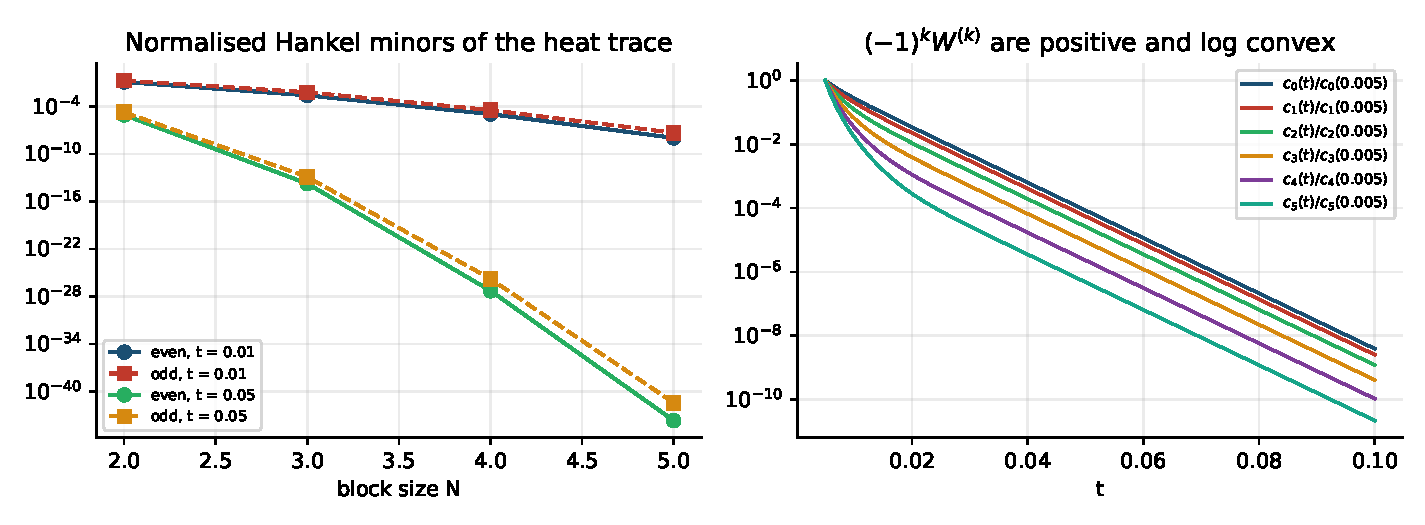
\includegraphics[width=\textwidth]{fig/hankel.pdf}
\caption{Left: normalised Hankel minors of the heat trace at two times; positivity persists but falls below any fixed precision as $t$ grows. Right: the first six $(-1)^kW^{(k)}(t)$, divided by their values at $t=0.005$, from $1700$ zeros.}
\label{fig:ch12:hankel}
\end{figure}

\begin{theorem}[{\cite[Theorem 7.10]{P17}}]\label{thm:ch12:cm}
Unconditionally, that is, using only the verification of RH below height $10^{12}$ \cite{PT21}, $(-1)^kW^{(k)}(t)>0$ for every $t>0$ and every integer $0\le k\le10^{17}$.
\end{theorem}

The proof again splits at $\tau$. Near the origin, Cauchy's estimate on a circle about $t$ of radius close to $t$, such as $(1-\frac1{k+1})t$, on which $\re(1/z)\ge1/(2t)$ and $|z|\ge t/(k+1)$, bounds the $k$th derivative of the prime term by a multiple of $(k+1)\Gamma(k+\frac12)t^{-k-\frac12}e^{-\kappa/t}$. Against $s_k(t)$ this loses a factor of order $k$ and gains $e^{-\kappa/t}\le e^{-1201}$, and for $k\ge1$ the archimedean term dominates by a margin of more than $2.9\,s_k(t)$, the case $k=0$ being Theorem~\ref{thm:ch12:idsd}. Away from the origin a zero in $(20,50]$ dominates all zeros above the verified height $H=10^{12}$, wherever they lie, provided $tH^2\ge2(k+1)$ and a logarithmic condition hold; Section~\ref{sec:ch12:reach} explains why these allow orders up to about $10^{18}$.

The Stieltjes moments of Table~\ref{tab:ch3:diag} give a Hankel test at the other end of the heat trace, and the test also returns the zeros \cite{P26wig}. They are the moments of $W$, $m_n=\frac1{n!}\int_0^\infty t^nW(t)\,dt=\sum_ja_j^{-n-1}$, and since $\log G(u)=\sum_j\log(1+u/a_j)=\sum_{n\ge1}(-1)^{n+1}m_{n-1}u^n/n$ they follow from the Taylor coefficients of $G(u)=\Xi(i\sqrt u)/\Xi(0)=\sum_kM_ku^k/((2k)!\,M_0)$, where $M_k=\int_\R v^{2k}\Phi(v)\,dv$; no zero enters. Under RH the $m_n$ are the moments of the positive measure $\nu=\sum_ja_j^{-1}\delta_{1/a_j}$, so every Hankel matrix $\mathcal H_N=[m_{i+j}]_{i,j<N}$ is positive definite. Conversely, if all of them are, Hamburger's theorem makes the $m_n$ the moments of a positive measure, of compact support because $|m_n|\le\sum_j|a_j|^{-n-1}$ grows at most geometrically, and then $\sum_nm_nw^n=\sum_j1/(a_j-w)$ has all its poles on the real axis: every $a_j$ is real, and positive because $\xi$ has no zeros in $(0,1)$, which is RH. The shifted matrices $\mathcal H'_N=[m_{i+j+1}]_{i,j<N}$ give the same test, and either suffices alone: if every $\mathcal H'_N$ is positive definite, Hamburger's theorem applied to $(m_{n+1})$ and $\sum_nm_nw^n=m_0+w\sum_nm_{n+1}w^n$ give the same conclusion. Positivity is tested by the Cholesky factorisation $\mathcal H_N=LL^\top$, and the factor gives more: $J_N=L^{-1}\mathcal H'_NL^{-\top}$ is the Jacobi matrix of $\nu$, tridiagonal, and its eigenvalues are the nodes of the $N$ point Gauss rule for $\nu$. They approximate the largest atoms $1/a_j$ first, so their inverse square roots return the lowest ordinates (Table~\ref{tab:ch12:jacobi}). With $M_0,\dots,M_{100}$ computed at $1000$ digits by the trapezoid rule, every $\mathcal H_N$ up to order $50$ is positive definite.

\begin{table}[htbp]
\centering\small
\begin{tabular}{rrllll}
\toprule
$N$ & zeros & error of $\gamma_1$ & last error & $\det\mathcal H_N/\det\mathcal H_{N-1}$ & digits\\
\midrule
$10$ & $2$ & $4.4\times10^{-18}$ & $1.3\times10^{-9}$ & $2.0\times10^{-61}$ & $60$\\
$20$ & $7$ & $1.6\times10^{-49}$ & $3.1\times10^{-7}$ & $1.2\times10^{-138}$ & $140$\\
$30$ & $12$ & $8.6\times10^{-87}$ & $2.4\times10^{-7}$ & $1.0\times10^{-221}$ & $230$\\
$40$ & $17$ & $6.1\times10^{-128}$ & $5.4\times10^{-8}$ & $1.3\times10^{-308}$ & $310$\\
$50$ & $22$ & $5.3\times10^{-172}$ & $5.4\times10^{-8}$ & $1.4\times10^{-398}$ & $400$\\
\bottomrule
\end{tabular}
\caption{The lowest ordinates from the Stieltjes moments $m_0,\dots,m_{2N-1}$, computed from the Taylor coefficients of $\Xi$ at the centre: the number returned by the Jacobi matrix of order $N$ to within $10^{-6}$, the errors of the first and of the last of them, the last Cholesky pivot of $\mathcal H_N$, and the least number of digits, in steps of $10$, of the Taylor coefficients and of the arithmetic from which on the same ordinates are returned.}
\label{tab:ch12:jacobi}
\end{table}

This is Gauss quadrature, equivalently Pad\'e approximation of $G'/G$ at the origin, and Table~\ref{tab:ch12:jacobi} shows its two limits. The first is precision. The last Cholesky pivot $\det\mathcal H_N/\det\mathcal H_{N-1}$ falls from $10^{-61}$ at $N=10$ to $10^{-398}$ at $N=50$, and the computation must resolve it. The precision thus grows linearly, by about $17$ digits for each further zero. The second is reach. An off line quadruple at height $\gamma$ enters $m_n$ with weight of order $\gamma^{-2n-2}$, against $\gamma_1^{-2n-2}$ for the first zero, so a block of order $N$ sees essentially only the zeros that its Gauss rule resolves; Section~\ref{sec:ch21:hankel} shows this along the de Bruijn Newman flow, where the order $30$ test registers the collision of the pair just above the zeros it resolves, and not a collision higher up. The program \texttt{jacobi\_zeros.py} computes the table.

The Hankel matrices count the zeros off the line as well as test RH. For a real polynomial this is a theorem attributed to Hermite \cite{Hermite1856}: the Hankel form of the power sums of the roots has as many negative squares as the polynomial has distinct pairs of nonreal roots. Let $\iota_N$ and $\iota'_N$ be the numbers of negative eigenvalues of $\mathcal H_N$ and $\mathcal H'_N$.

\begin{theorem}\label{thm:ch12:inertia}
Let $K\in\{0,1,2,\dots\}\cup\{\infty\}$ be the number of distinct zeros $\rho$ of $\xi$ with $\re\rho>\frac12$ and $\im\rho>0$. Then $\iota_N$ and $\iota'_N$ are nondecreasing in $N$, $\iota_N\le K$ and $\iota'_N\le K$ for every $N$, and $\iota_N\to K$ and $\iota'_N\to K$ as $N\to\infty$. In particular RH holds if and only if $\iota_N=0$ for every $N$, and if it fails, $\iota_N\ge1$ from some $N$ on; the same holds for $\iota'_N$.
\end{theorem}

\begin{proof}
Put $b_k=1/a_k$, listed with multiplicity, so that $m_n=\sum_kb_k^{n+1}$ and $\sum_k|b_k|<\infty$. For a real vector $x=(x_0,\dots,x_{N-1})$ and $P(w)=\sum_ix_iw^i$,
\[
x^\top\mathcal H_Nx=\sum_kb_kP(b_k)^2,\qquad x^\top\mathcal H'_Nx=\sum_kb_k^2P(b_k)^2,
\]
the sums converging absolutely. A zero on the line gives $b_k=\gamma_k^{-2}>0$ and nonnegative terms. A zero $\rho=\frac12+\delta+i\gamma$ with $\delta>0$ and $\gamma>0$, of multiplicity $\mu$, gives $a=-(\delta+i\gamma)^2$ with $\im a=-2\delta\gamma<0$, hence $b=1/a$ with $\im b>0$; its mirror image $1-\bar\rho$ gives $\bar a$ and $\bar b$ with the same multiplicity, and since $P$ has real coefficients the two contribute $2\mu\re\big(bP(b)^2\big)$ to the first form. With $u=\re P(b)$ and $v=\im P(b)$ this is $2\mu\big(\re b\,(u^2-v^2)-2\im b\,uv\big)$, a quadratic form in $(u,v)$ whose matrix has determinant $-4\mu^2|b|^2<0$, so it has exactly one negative square, and composed with the linear map $x\mapsto(u,v)$ it has at most one. The terms of the zeros on the line add up to a positive semidefinite form, so $\iota_N\le K$. In the second form the weight is $b^2$, and $2\mu\re\big(b^2P(b)^2\big)$ is again a form in $(u,v)$ of determinant $-4\mu^2|b|^4<0$, so $\iota'_N\le K$. Since $\mathcal H_N$ is the leading principal submatrix of $\mathcal H_{N+1}$, Cauchy's interlacing theorem shows that $\iota_N$ does not decrease, and the same holds for $\iota'_N$.

For the lower bound let $\mathcal B$ be the closure of $\{b_k\}$. It is a countable compact set, symmetric under conjugation, whose only possible accumulation point is $0$, and a countable compact set does not separate the plane, so $\C\setminus\mathcal B$ is connected. Fix a finite $m\le K$ and distinct atoms $\omega_1,\dots,\omega_m$ with $\im\omega_j>0$, of multiplicities $\mu_j$; they are isolated points of $\mathcal B$. On $\C^m=\R^{2m}$ the form $q(y)=\sum_{j\le m}2\mu_j\re(\omega_jy_j^2)$ is a sum of $m$ forms in the pairs $(\re y_j,\im y_j)$, each with one negative square, so there are an $m$ dimensional real subspace $E$ and $\lambda_0>0$ with $q(y)\le-\lambda_0|y|^2$ on $E$. Let $y^{(1)},\dots,y^{(m)}$ be a basis of $E$ and $\lambda_1>0$ such that $|\sum_i\alpha_iy^{(i)}|^2\ge\lambda_1|\alpha|^2$ for $\alpha\in\R^m$. Take open discs $D_j$ about $\omega_j$, and their mirror images $D_j^*$ about $\bar\omega_j$, whose closures are disjoint and meet $\mathcal B$ only in their centres, and an open set $O\supset\mathcal B\setminus\{\omega_1,\bar\omega_1,\dots,\omega_m,\bar\omega_m\}$, symmetric under conjugation and disjoint from the closed discs, which exists because that set is compact. Let $f_i$ be $y^{(i)}_j$ on $D_j$, $\overline{y^{(i)}_j}$ on $D_j^*$ and $0$ on $O$. Each $f_i$ is holomorphic on a neighbourhood of $\mathcal B$, so by Runge's theorem there are polynomials $\tilde P_i$ with $|\tilde P_i-f_i|<\varepsilon$ on $\mathcal B$, and since $\mathcal B$ and $f_i$ are symmetric under conjugation, $P_i(w)=\frac12\big(\tilde P_i(w)+\overline{\tilde P_i(\bar w)}\big)$ has real coefficients and satisfies the same bound. For $\alpha\in\R^m$ and $P=\sum_i\alpha_iP_i$ we have $|P(b_k)|\le\varepsilon\sqrt m\,|\alpha|$ at every atom other than the $\omega_j$ and $\bar\omega_j$, and $P(\omega_j)=\sum_i\alpha_iy^{(i)}_j+\eta_j$ with $|\eta_j|\le\varepsilon\sqrt m\,|\alpha|$. The atoms $\omega_j$ and $\bar\omega_j$ contribute $\sum_j2\mu_j\re\big(\omega_jP(\omega_j)^2\big)$ to the first form, so for $\varepsilon\le1$ and a constant $C$ that depends on neither $\varepsilon$ nor $\alpha$,
\[
\sum_kb_kP(b_k)^2\le q\Big(\sum_i\alpha_iy^{(i)}\Big)+C\varepsilon|\alpha|^2\le-(\lambda_0\lambda_1-C\varepsilon)|\alpha|^2 .
\]
For $\varepsilon<\lambda_0\lambda_1/C$ the right side is negative for $\alpha\ne0$, so the coefficient vectors of $P_1,\dots,P_m$ span an $m$ dimensional space on which the form of $\mathcal H_N$ is negative definite as soon as $N$ exceeds their degrees, and $\iota_N\ge m$ for those $N$. For $\mathcal H'_N$ the same argument applies with $\omega_j^2$ in place of $\omega_j$ in $q$ and the weights $b_k^2$ in the sum. Since $m\le K$ is arbitrary, $\iota_N\to K$ and $\iota'_N\to K$.
\end{proof}

In determinant form the theorem is classical. For a real entire function of order one with zeros $z_j$, Grommer \cite{Grommer14} proved that all its zeros are real if and only if the determinants $D_n=\det(s_{i+j})_{i,j<n}$ of the power sums $s_k=\sum_jz_j^{-k-2}$ are positive for every $n\ge1$, and Chebotarev \cite{Chebotarev28} that if the sequence $D_{n-1}D_n$, $n\ge1$, with $D_0=1$, has exactly $m$ negative terms, the function has $m$ distinct pairs of complex conjugate zeros; Baricz and \v{S}tampach state both in this form \cite[Theorem 10]{BS18}. For $\Xi$, whose zeros are the square roots of the $a_k$, $s_{2l}=2m_l$ and $s_{2l+1}=0$, so after the even indices are put first $(s_{i+j})_{i,j<n}$ is block diagonal with the blocks $2\mathcal H_{\lceil n/2\rceil}$ and $2\mathcal H'_{\lfloor n/2\rfloor}$, whose negative indices add up to $\iota_{\lceil n/2\rceil}+\iota'_{\lfloor n/2\rfloor}$; this tends to $2K$, and each zero $\rho$ counted by $K$ gives two pairs of complex conjugate zeros of $\Xi$, as Chebotarev's count requires. Counting by eigenvalues rather than by the signs of determinants, Theorem~\ref{thm:ch12:inertia} needs no determinant to be nonzero, allows $K=\infty$ and holds for each family separately. Along the de Bruijn Newman flow the proof applies at every time to the zeros of $H_t$, none of which is purely imaginary (Section~\ref{sec:ch21:hankel}).

\subsection{Every order near the origin}\label{sec:ch12:allorders}

Let $s_k(t)=\Gamma(k+\frac12)t^{-k-\frac12}/(4\pi)$ as in the proof of Theorem~\ref{thm:ch12:idsd}, let $E_k(t)$ be the average of $m$ against the weight $r^{2k}e^{-r^2t}$ on $[0,\infty)$, and let $F_k(x)={}_1F_1(k+\frac12;\frac12;-x^2)$. Expanding the cosine in its power series gives $\frac1{2\pi}\int_{\R}r^{2k}e^{-r^2t}\cos(ry)\,dr=2s_k(t)F_k(y/2\sqrt t)$, whose case $k=0$ is the kernel $e^{-y^2/4t}/(2\sqrt{\pi t})$ of the prime term of \eqref{eq:ch2:Warith}. Differentiating \eqref{eq:ch2:Warith} $k$ times term by term, which the Gaussian factors in $r$ and in $\log n$ allow, therefore gives, with no hypothesis on the zeros,
\begin{equation}\label{eq:ch12:ckarith}
\frac{c_k(t)}{s_k(t)}=E_k(t)-2\sum_{n\ge2}\frac{\Lambda(n)}{\sqrt n}F_k(x_n)+\frac{(-\frac14)^ke^{t/4}}{s_k(t)},\qquad x_n=\frac{\log n}{2\sqrt t}.
\end{equation}
In \eqref{eq:ch12:ckarith} the archimedean term $E_k(t)$ grows with $k$.

\begin{lemma}\label{lem:ch12:hermite}
\textup{(a)} For every integer $k\ge0$ and every $x\ge0$, $|F_k(x)|\le B(x)e^{-x^2/2}$, where $B(x)=\max\{2.62,\ (\pi(2ex^2+\frac12))^{1/4}\}$.

\textup{(b)} Let $0<\varepsilon<1$, and let $k\ge1$ and $x\ge0$ satisfy $e^2x^2\le4\varepsilon k$. Then $|F_k(x)|\le C_\varepsilon(k)e^{-x^2/2}$, where $C_\varepsilon(k)=\sqrt{(k+0.37)/((1-\varepsilon)k+\frac14)}+2\sqrt{k+0.37}\,e^{-\varepsilon k}$.
\end{lemma}

\begin{proof}
Taking $t=1$ and $y=2x$ above, $F_k(x)=\Gamma(k+\frac12)^{-1}\int_{\R}r^{2k}e^{-r^2+2ixr}\,dr$. Put $\mu=x^2/4$. The integrand is entire and decays in every horizontal strip, so the path can be moved to $\im r=x/2$, where $|r^{2k}|=(\sigma^2+\mu)^k$, $|e^{-r^2}|=e^{-\sigma^2+\mu}$ and $|e^{2ixr}|=e^{-4\mu}$, with $\sigma=\re r$. Expanding $(\sigma^2+\mu)^k$ by the binomial theorem gives, for every $k$ and $x$,
\[
|F_k(x)|\le e^{-3\mu}\sum_{j=0}^k\frac{\mu^j}{j!}P_{k,j},\qquad P_{k,j}=\frac{\Gamma(k+1)}{\Gamma(k+\frac12)}\,\frac{\Gamma(k-j+\frac12)}{\Gamma(k-j+1)}.
\]
Kershaw's inequalities $\sqrt{y+\frac14}\le\Gamma(y+1)/\Gamma(y+\frac12)\le\sqrt{y+0.37}$, proved for $y>0$ in \cite{Kershaw83} and true at $y=0$, where the ratio is $1/\sqrt\pi$, give $P_{k,j}\le\sqrt{(k+0.37)/(k-j+\frac14)}$, which is less than $\sqrt2$ for $j\le k/2$ and at most $2\sqrt{k+0.37}$ for every $j$. For (a), suppose first that $k\ge2ex^2$. Since $k/2\ge4e\mu$, Chernoff's bound $\sum_{j\ge a}\mu^j/j!\le(e\mu/a)^a$ for the Poisson law, valid for $a>\mu$, gives $\sum_{j\ge k/2}\mu^j/j!\le(2e\mu/k)^{k/2}\le2^{-k}$, and $2\sqrt{k+0.37}\,2^{-k}\le\sqrt{1.37}<1.2$ for $k\ge1$. Hence $|F_k(x)|\le e^{-3\mu}(\sqrt2\,e^\mu+1.2)\le(\sqrt2+1.2)e^{-x^2/2}$, and $\sqrt2+1.2<2.62$; for $k=0$ the assumption forces $x=0$, where $F_0=1$.

Suppose now that $k<2ex^2$. Kummer's transformation and the Hermite case of ${}_1F_1$ \cite[(13.2.39), (13.6.16)]{DLMF} give $F_k(x)=e^{-x^2}{}_1F_1(-k;\frac12;x^2)=(-1)^k\frac{k!}{(2k)!}e^{-x^2}H_{2k}(x)$, and the bound $e^{-x^2/2}|H_n(x)|\le(2^nn!)^{1/2}$ \cite[(18.14.9)]{DLMF} gives
\[
|F_k(x)|\le\Big(\frac{4^k(k!)^2}{(2k)!}\Big)^{1/2}e^{-x^2/2}\le\big(\pi(k+\tfrac12)\big)^{1/4}e^{-x^2/2}<\big(\pi(2ex^2+\tfrac12)\big)^{1/4}e^{-x^2/2},
\]
since $4^k(k!)^2/(2k)!=\sqrt\pi\,\Gamma(k+1)/\Gamma(k+\frac12)\le\sqrt{\pi(k+\frac12)}$ by Kershaw's upper bound.

For (b), split the sum at $j=\varepsilon k$ instead. For $j\le\varepsilon k$, $P_{k,j}\le\sqrt{(k+0.37)/((1-\varepsilon)k+\frac14)}$, and these $j$ contribute at most that times $e^\mu$. For $j>\varepsilon k$, $P_{k,j}\le2\sqrt{k+0.37}$, and since $\varepsilon k\ge e^2\mu>\mu$, Chernoff's bound gives $\sum_{j\ge\varepsilon k}\mu^j/j!\le(e\mu/\varepsilon k)^{\varepsilon k}\le e^{-\varepsilon k}$. Hence $|F_k(x)|\le e^{-3\mu}\big(\sqrt{(k+0.37)/((1-\varepsilon)k+\frac14)}\,e^\mu+2\sqrt{k+0.37}\,e^{-\varepsilon k}\big)\le C_\varepsilon(k)e^{-x^2/2}$.
\end{proof}

\begin{theorem}\label{thm:ch12:cmint}
\textup{(a)} For every integer $k\ge1$ and every $t\in(0,0.019]$, $(-1)^kW^{(k)}(t)>0$. The proof uses no information on the zeros.

\textup{(b)} Unconditionally, that is, using only the verification of RH below height $10^{12}$ \cite{PT21}, $W$ is completely monotone on $(0,1.29]$: $(-1)^kW^{(k)}(t)>0$ for every $t\in(0,1.29]$ and every integer $k\ge0$.
\end{theorem}

\begin{proof}
By \eqref{eq:ch12:ckarith} and Lemma~\ref{lem:ch12:hermite}(a), for every $k\ge0$ and $t>0$,
\[
\frac{c_k(t)}{s_k(t)}\ge E_k(t)-S_B(t)-Q_k(t),
\]
where
\[
S_B(t)=2\sum_{n\ge2}\frac{\Lambda(n)}{\sqrt n}B(x_n)e^{-(\log n)^2/8t},\qquad Q_k(t)=\frac{4\pi e^{t/4}t^{k+\frac12}}{4^k\,\Gamma(k+\frac12)}.
\]
Above the order $K=10^{17}$ part (b) of the lemma does better. Take $\varepsilon=10^{-6}$. The first term of $C_\varepsilon(k)$ decreases in $k$, because $\frac14<0.37(1-\varepsilon)$, and the second decreases for $k>1/(2\varepsilon)$, so $C_\varepsilon(k)\le C=C_\varepsilon(K+1)<1+6\times10^{-7}$ for $k>K$, and $e^2x^2\le4\varepsilon k$ holds for $x\le2\sqrt{\varepsilon(K+1)}/e$, which exceeds $2.3\times10^5$. For $t\ge0.019$ every prime power $n\le2^{24}$ has $x_n<61$. So for $k>K$ and $t\ge0.019$ the bound holds with $S_B$ replaced by $S_C$, the sum $S_B$ with $B(x_n)$ replaced by $C$ for $n\le2^{24}$.

The three terms are monotone. Since $m$ increases on $[0,\infty)$, and the weights $r^{2k}e^{-r^2t}$ have likelihood ratios $r^2$ from $k$ to $k+1$ and $e^{r^2(t'-t)}$ from $t'$ to $t<t'$, both increasing in $r$, $E_k(t)$ increases in $k$ and decreases in $t$. $Q_k(t)$ increases in $t$, and for $t\le2$ it decreases in $k$, the ratio of consecutive terms being $t/(4k+2)$. $B(x)e^{-x^2/2}$ decreases on $(0,\infty)$: the second branch of $B$ increases and is $1.78$ at $x=2^{-1/2}$, so $B=2.62$ below that point, and above it the logarithmic derivative of the second branch times $e^{-x^2/2}$ is less than $1/(2x)-x<0$; since $x_n$ decreases in $t$, $S_B$ and $S_C$ increase in $t$. So for $k\ge k_0$ and $t\le T\le2$ each bound is at least its value at $(k_0,T)$, and it suffices to prove $E_1(0.019)-S_B(0.019)-Q_1(0.019)>0$, which gives (a), and $E_{K+1}(1.29)-S_C(1.29)-Q_{K+1}(1.29)>0$, which gives the orders $k>K$ on $[0.019,1.29]$; with (a) for $t\le0.019$ and Theorem~\ref{thm:ch12:cm} for the orders $k\le K$, this gives (b).

For the first, lower sums over $[0,64]$, which the monotonicity of $m$ allows, and the positivity of $m$ beyond $64$ give $E_1(0.019)>0.15924$; the prime powers $n\le30000$ and the tail bound below give $S_B(0.019)<0.13628$; and $Q_1(0.019)<0.00933$. For the second, the weight $r^{2K+2}e^{-r^2t}$ makes $v=r^2t$ a gamma variable of shape $\lambda=K+\frac32$, and Chernoff's bound for the gamma law, $\Pr(v<a)\le(a/\lambda)^\lambda e^{\lambda-a}$ for $a<\lambda$, gives $\Pr(v<a)<e^{-1000}$ for $a=(1-2^{-13})^2\lambda$. As $m$ increases, $E_{K+1}(t)\ge m(r_1)-(m(r_1)-m(0))e^{-1000}$ with $r_1=\sqrt{a/t}$, which gives $E_{K+1}(1.29)>17.6066$; the prime powers $n\le2^{24}$ and the tail bound below give $S_C(1.29)<17.5848$; and $Q_{K+1}(1.29)<e^{-1000}$. In both cases the prime powers above the cutoff $n_0$, which is $30000$ and $2^{24}$, add less than $2\big(2.62+2.08(2\sqrt t)^{-1/2}\big)n_0^{1-q}/(q-1)$ with $q=\log n_0/8t$, because $x_n\ge x_{n_0}\ge1$ and $e^{-(\log n)^2/8t}\le n^{-q}$ for $n>n_0$, $B(x)\le2.62+2.08\sqrt x$ for $x\ge1$, and $\log n$ and $(\log n)^{3/2}$ are at most $\sqrt n$ for $n\ge e^{10}$; this is below $10^{-299}$ and $5\times10^{-4}$. The program \texttt{cm\_orders.py} evaluates every numerical inequality of this proof and of the proof of Lemma~\ref{lem:ch12:hermite} in ball arithmetic.
\end{proof}

Computed in floating point, the bound $E_1-S_B-Q_1$ of (a) vanishes at $t=0.0193$; $E_1$ itself vanishes at $t=0.0261$, so no bound on the size of the prime terms carries (a) much further. Part (b) goes further because $E_k(t)=\frac12(\psi(k+\frac12)-\log t)-\log2\pi+O(t/k)$ grows like $\frac12\log k$, while at such orders part (b) of the lemma bounds the prime terms at almost no cost: the bound $E_{K+1}-S_C$, computed in the same way, vanishes at $t=1.2912$, while $E_{K+1}-S_B$ vanishes at $t=0.578$.

The ray of Section~\ref{sec:ch12:ray} shows what the proof uses. On the ray $t=k/u^2$, $e^{-f_0}c_k(t)$ is to leading order the Gaussian smoothing $\mathcal G(u,t)$ of the zeros (Proposition~\ref{prop:ch12:ray}), $E_k(t)$ is close to $\log(u/2\pi)$, and for large $k$ the factor $F_k(x_n)$ is close to $e^{-(\log n)^2/8t}\cos(u\log n)$. The proof is therefore the bound of Section~\ref{ch:lessons} that ignores the phases of the primes, made uniform in the order; with $C$ replaced by one, $S_C$ is twice the sum $S$ of that section, up to the prime powers above $2^{24}$. Above the order $10^{17}$ uniformity costs a factor below $1+6\times10^{-7}$, so $1.2912$, the root of $E_{K+1}(t)=2S(t)$, is as far as this argument can carry (b) with $K=10^{17}$: it bounds the prime terms by one envelope for all orders above $K$, and the archimedean term by its value at the order $K+1$. A bound that ignores the phases but treats the orders separately is not covered by this limit. At low orders it costs the factor $B\ge2.62$ of part (a), and part (a) is not sharp: on a grid of $0.5\le x\le20$ and $k\le1200$ the ratio $|F_k(x)|e^{x^2/2}/B(x)$ is at most $0.44$ (computed). The ray also says where (b) looks. To leading order, complete monotonicity on $(0,T]$ asks for positive Gaussian smoothings at resolutions $1/(2\sqrt t)$ of at least $1/(2\sqrt T)$, which is $0.44$ for $T=1.29$, finer than the $0.46$ at which the quadruples of Table~\ref{tab:ch13:first}, at distance $\frac14$ from the line, first make the smoothing negative, at $t=1.18$. There is no conflict, because the orders above $10^{17}$ at $t\le1.29$ lie on the rays at heights $u=\sqrt{k/t}>2.78\times10^8$, where the time $t_0(u)$ of Section~\ref{ch:lessons}, below which the phase free bound makes the smoothing positive whatever the zeros, exceeds $1.29$. The quadruples lie below height $2000$, at heights where $t_0$ is at most $0.511$, and there (b) rests on the verified zeros, through Theorem~\ref{thm:ch12:cm}.

\subsection{Williamson measures: the Thorin measure smoothed by gamma laws}\label{sec:ch12:kmono}

Complete monotonicity is the limit of $k$ monotonicity, which asks only that the first $k$ derivatives alternate in sign, and by Williamson's theorem \cite{Williamson} a $k$ monotone function that vanishes at infinity is a positive mixture of the truncated powers $(1-tz/k)_+^{k-1}$. For the heat trace the mixing measure is explicit,
\[
W(t)=\int_0^\infty\Big(1-\frac{tz}k\Big)_+^{k-1}U_k(dz),\qquad U_k(dz)=\frac{k^k}{(k-1)!}z^{-k-1}c_k\Big(\frac kz\Big)dz,
\]
and we call $U_k$ the Williamson measure of order $k$. By Theorem~\ref{thm:ch12:cm} it is positive for every $k\le10^{17}$ \cite[Corollary 7.13]{P17}, and by Theorem~\ref{thm:ch12:window} for every $k\le1.16\times10^{25}$. RH holds if and only if $U_k\ge0$ for infinitely many $k$, since then $W$ is $k$ monotone for infinitely many $k$, hence completely monotone.

The summands of $U_k$ are inverse gamma laws, by an elementary identity: for $k\ge1$ and $c\ge0$,
\begin{equation}\label{eq:ch12:gammak}
e^{-c}=\E\Big(1-\frac c{\Gamma_k}\Big)_+^{k-1},\qquad \Gamma_k\sim\mathrm{Gamma}(k,1),
\end{equation}
since $\int_c^\infty(\omega-c)^{k-1}e^{-\omega}d\omega/\Gamma(k)=e^{-c}$. With $c=a_jt$ and $z=ka_j/\Gamma_k$, so that $1-a_jt/\Gamma_k=1-tz/k$, the identity shows that $U_k$ is the sum over the zeros of the densities $(ka_j)^kz^{-k-1}e^{-ka_j/z}/(k-1)!$. For real $a_j$ this is the inverse gamma law of $ka_j/\Gamma_k$. Under RH, therefore, writing $\mathcal L(Y)$ for the law of $Y$,
\[
U_k=\sum_\gamma\mathcal L\Big(\gamma^2\,\frac k{\Gamma_k}\Big),
\]
a sum of probability laws: the Thorin measure with each atom $\gamma^2$ spread over a relative width of about $1/\sqrt k$. As $k\to\infty$ the ratio $\Gamma_k/k$ concentrates at one and the atoms reappear, which is the passage from Williamson's theorem to Bernstein's; in statistics, Polson, Scott and Windle used $k$ monotone mixtures of this kind to build samplers for the Bayesian bridge \cite[Section 2.2, Theorem 2.1]{PSW14} and noted the same limit \cite[Section 3]{PSW14}.

The Williamson measures form a second resolution family for the Thorin measure, beside the Poisson family $\rho_\varepsilon$, which is the Cauchy flow of Section~\ref{ch:clock}. In the chart $\theta=\sqrt z$ the gamma smoothing spreads the atom at $\gamma$ over a width of about $\gamma/(2\sqrt k)$, proportional to the height, while the Poisson smoothing spreads every atom over the width $\varepsilon$, and the inverse gamma kernel has tails far lighter than the $x^{-2}$ tails of the Cauchy kernel. In Figure~\ref{fig:ch12:kmono}, where the widths match at $\theta=30$, the Williamson densities fall by many orders of magnitude between neighbouring zeros and the Poisson densities by only one to four.

\begin{figure}[htbp]
\centering
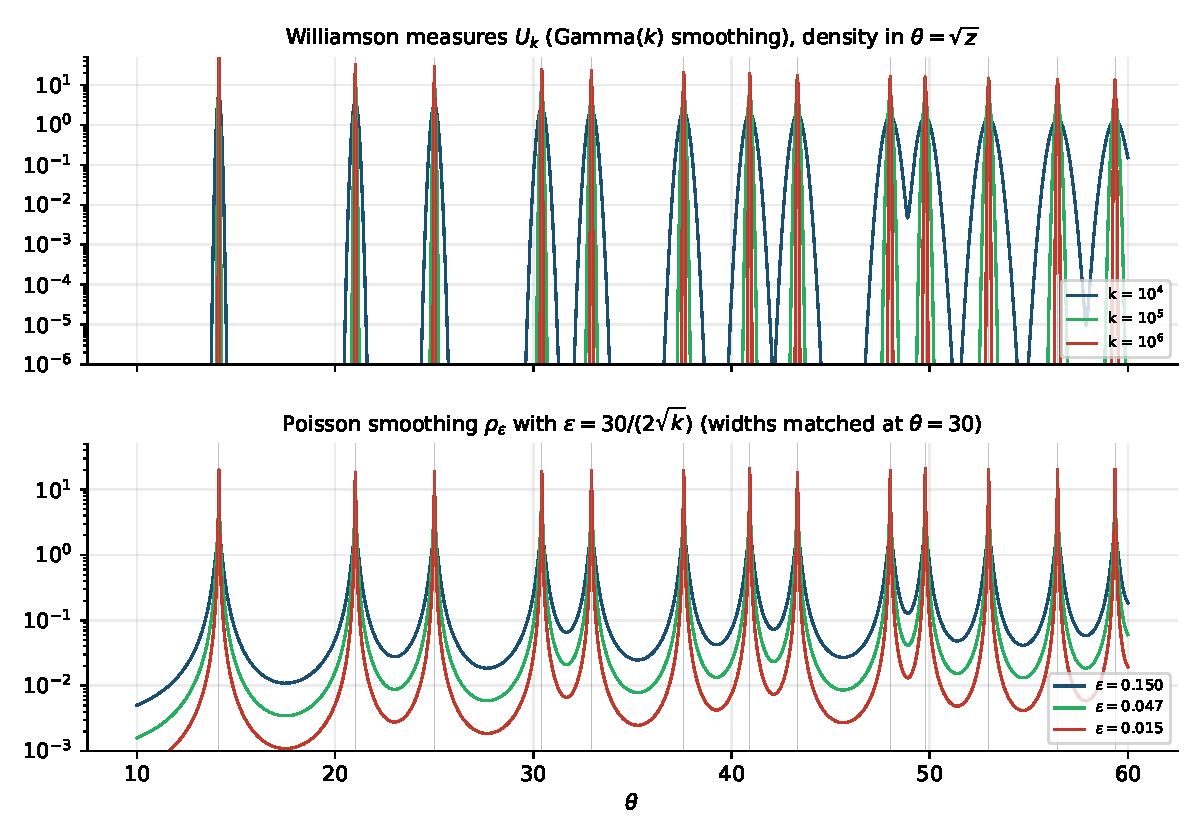
\includegraphics[width=0.95\textwidth]{fig/kmono.pdf}
\caption{Top: the Williamson measures $U_k$ of the heat trace for $k=10^4$, $10^5$, $10^6$, computed from $1700$ zeros, as densities in $\theta=\sqrt z$. Bottom: the Poisson smoothed Thorin densities $\rho_\varepsilon$ with $\varepsilon=30/(2\sqrt k)$, so that the widths match at $\theta=30$.}
\label{fig:ch12:kmono}
\end{figure}

The Poisson smoothing of the zeros is $\pi^{-1}\re(\xi'/\xi)$ off the line and can be computed from $\xi$ alone at every resolution, which is why $\rho_\varepsilon$ is the central object of Chapter~\ref{chap:measure} and Section~\ref{ch:weak}; the price is the heavy tail, which makes positivity at one resolution a statement about all zeros at once. The gamma smoothing is local, and an off line pair contributes to $U_k$ a signed, oscillating term near its height.

\subsection{Along a ray: the Gaussian smoothing of the zeros}\label{sec:ch12:ray}

Fix a height $u$ and move along the ray $t=k/u^2$ of the $(k,t)$ plane, on which the weight $x^ke^{-xt}$ of $c_k(t)$ peaks at $x=u^2$ and the density of $U_k$ is taken at $z=u^2$. Write each zero as $\rho=\frac12+\delta+i\gamma$ and put $\tilde\gamma=\gamma-i\delta$, so that $a=\tilde\gamma^2$; as in every sum of this section, the zero is taken with $\gamma>0$ from each pair $\{\rho,1-\rho\}$. The Gaussian smoothing of the zeros at resolution $1/(2\sqrt t)$ is
\[
\mathcal G(u,t)=\sum e^{-2t(\tilde\gamma-u)^2}.
\]
A zero on the line contributes a Gaussian bump at its ordinate. The zeros $\frac12\pm\delta+i\gamma$ of a quadruple $\frac12\pm\delta\pm i\gamma$ have conjugate values of $\tilde\gamma$, so $\mathcal G$ is real, and together they contribute $2e^{2t(\delta^2-(\gamma-u)^2)}\cos(4t\delta(\gamma-u))$, a bump amplified by $e^{2t\delta^2}$ and modulated in $u$ with period $\pi/(2t\delta)$. At $u=0$, $\mathcal G(0,t)=W(2t)$.

\begin{proposition}\label{prop:ch12:ray}
Let $u\ge2$, $t>0$ and $k=u^2t$, not necessarily an integer, with $a^k$ the principal power in $c_k(t)=\sum a^ke^{-at}$, and let $f_0=k(\log u^2-1)$. Then
\[
e^{-f_0}c_k(t)=\sum_{|\tilde\gamma-u|\le u/2}e^{-2t(\tilde\gamma-u)^2}\big(1+\varepsilon_\rho\big)+R,\qquad |\varepsilon_\rho|\le\exp\Big\{\frac{4t}{3u}|\tilde\gamma-u|^3\Big\}-1,
\]
where, with $\ell_\pm=u\pm\frac12\sqrt{u^2-1}$, $H(r)=u^2\log\frac{r^2+1/4}{u^2}-r^2+\frac14+u^2$ and $\eta=1-u^2/(\ell_+^2+\frac14)>0$,
\[
|R|\le N(\ell_-)e^{tH(\ell_-)}+\Big(\ell_+^2+\frac1{t\eta}\Big)e^{tH(\ell_+)}.
\]
No hypothesis on the zeros is used.
\end{proposition}

\begin{proof}
Put $\tilde\gamma=u+v$ and $w=v/u$. Since $\re\tilde\gamma>0$ and $|\arg\tilde\gamma|<\frac\pi4$, the principal logarithm gives $e^{-f_0}a^ke^{-at}=e^E$ with
\[
E=tu^2\big(2\log(1+w)-2w-w^2\big)=-2tv^2+2tu^2\sum_{m\ge3}\frac{(-1)^{m+1}w^m}m ,
\]
and for $|w|\le\frac12$ the series has modulus at most $|w|^3/(3(1-|w|))\le\frac23|w|^3$. This gives $\varepsilon_\rho=e^{E+2tv^2}-1$ and its bound, since $|e^z-1|\le e^{|z|}-1$. For a zero with $|v|>u/2$, $|v|^2=(\gamma-u)^2+\delta^2$ and $\delta^2<\frac14$ give $|\gamma-u|>\frac12\sqrt{u^2-1}$, so that $\gamma<\ell_-$ or $\gamma>\ell_+$, and $|e^E|=\exp t\big(u^2\log(|a|/u^2)-\re a+u^2\big)\le e^{tH(\gamma)}$, because $|a|=\gamma^2+\delta^2$ and $\re a=\gamma^2-\delta^2$. The function $H$ increases up to $\sqrt{u^2-\frac14}$, which lies between $\ell_-$ and $\ell_+$, so each of the at most $N(\ell_-)$ zeros below $\ell_-$ contributes at most $e^{tH(\ell_-)}$. For $r\ge\ell_+$, $\log(1+x)\le x$ gives $H(r)\le H(\ell_+)-\eta(r^2-\ell_+^2)$. The explicit Riemann von Mangoldt formula \cite[Corollary~1.2]{HSW22} gives $N(r)\le r^2$ for every $r$, and partial summation then gives $\sum_{\gamma>\ell_+}e^{-q(\gamma^2-\ell_+^2)}\le\ell_+^2+1/q$ for $q>0$; take $q=t\eta$.
\end{proof}

For $u\ge10$ the ratios $H(\ell_-)/u^2$ and $H(\ell_+)/u^2$ decrease in $u$, from $-0.616$ and $-0.431$ at $u=10$, and $\eta>0.55$, so that $|R|\le(3u^2+2/t)e^{-0.43k}$. What remains is $\varepsilon_\rho$, whose term of order $1/u$ is $\frac{2t}{3u}(\tilde\gamma-u)^3$. Along the ray, therefore, $e^{-f_0}c_k(t)$ is $\mathcal G(u,t)$ up to an exponentially small remainder and, in each term, a relative error at most $e^{4t|\tilde\gamma-u|^3/3u}-1$. That error is small, of order $t|\tilde\gamma-u|^3/u$, for the terms that carry the sum provided $t|\tilde\gamma-u|^3$ is small against $u$ for them; for the zeros within a few multiples of $1/\sqrt t$ of $u$ it is of order $1/(\sqrt t\,u)$. It is not small in general: at a fixed height, as $t$ grows, the term of the nearest zero dominates, and its relative error grows with $t$. For an integer $k$ the density of $U_k$ in the chart $\theta=\sqrt z$ is exactly $\sqrt{2t/\pi}\,e^{-\lambda_k}e^{-f_0}c_k(t)$ at $\theta=u$, where $t=k/u^2$ and $\lambda_k\in(\frac1{12k+1},\frac1{12k})$ is the remainder in Stirling's formula for $k!$ \cite{Robbins55}. The density of $U_k$ at $\theta$ is therefore about $\sqrt{2t/\pi}\,\mathcal G(\theta,t)$ with $t=k/\theta^2$: the zeros smoothed by normal densities of standard deviation $1/(2\sqrt t)=\theta/(2\sqrt k)$, which is the width found above.

\begin{proposition}\label{prop:ch12:gauss}
RH holds if and only if $\mathcal G(u,t)\ge0$ for every real $u$ and every $t>0$.
\end{proposition}

\begin{proof}
Under RH every term is positive. Suppose that $\frac12+d+ic$ is a zero with $d>0$, and let $|u-c|<\frac d2$. The term of a zero has modulus $e^{2t\phi}$ with $\phi=\delta^2-(\gamma-u)^2$. For the zero $\frac12+d+ic$, $\phi>\frac34d^2$; for a zero with $|\gamma-c|>1$, $\phi<\frac14-\frac9{16}<0$. Group the finitely many zeros with $|\gamma-c|\le1$ by their type $(\gamma,|\delta|)$. Two types at the same ordinate have exponents $\phi$ differing by a nonzero constant, and two at different ordinates have exponents differing by a nonconstant affine function of $u$, so outside finitely many points one type has the largest $\phi$. Fix such a $u_*$, different from every ordinate, and let $(\gamma_*,d_*)$ be the maximising type and $\phi_*$ its exponent. Then $\phi_*>\frac34d^2$, so $d_*>0$, and the type consists of $\nu\ge2$ zeros counted with multiplicity, which contribute $\nu e^{2t\phi_*}\cos(4td_*(\gamma_*-u_*))$. Along $t_j=(2j+1)\pi/(4d_*|\gamma_*-u_*|)$ this is $-\nu e^{2t_j\phi_*}$. The other $n$ zeros with $|\gamma-c|\le1$ contribute at most $ne^{2t_j(\phi_*-\Delta)}$, with $\Delta>0$ the gap to the next exponent, and the zeros with $|\gamma-c|>1$ at most $32\log(c+2)e^{-5t_j/8}$ once $t_j\ge1$, since by the explicit Riemann von Mangoldt formula every interval of heights $[y,y+1]$ holds at most $4\log(y+3)$ zeros. Hence
\[
e^{-2t_j\phi_*}\mathcal G(u_*,t_j)\le-\nu+ne^{-2t_j\Delta}+32\log(c+2)e^{-(2\phi_*+5/8)t_j},
\]
which is negative for all large $j$.
\end{proof}

\begin{proposition}\label{tx:prop:offline}
For $\frac12<\alpha<1$ let $\eta=\alpha-\frac12$ and $\mathcal G_\alpha(u,t)=\re\sum e^{-2t(\tilde\gamma+i\eta-u)^2}$, over the zeros with $\gamma>0$ as for $\mathcal G$, which is $\mathcal G$ at $\eta=0$. Under RH $\mathcal G_\alpha(u,t)<0$ for some $u$ and $t$: there is no Gaussian criterion on the line $\re s=\alpha$.
\end{proposition}

\begin{proof}
Under RH $\tilde\gamma=\gamma$, and the term of $\gamma$ is $e^{2t\eta^2}e^{-2t(\gamma-u)^2}\cos\big(4t\eta(\gamma-u)\big)$. Take $u=\gamma_1+\pi/(4t\eta)$, where $\gamma_1$ is the lowest ordinate and a simple zero, and let $g>0$ be the gap to the next ordinate. The term of $\gamma_1$ is $-e^{2t\eta^2-\pi^2/(8t\eta^2)}$. For $t\ge\pi/(2\eta g)$ every other $\gamma$ has $\gamma-u\ge(\gamma-\gamma_1)/2$, so the other terms total at most $e^{2t\eta^2}\sum_{\gamma>\gamma_1}e^{-t(\gamma-\gamma_1)^2/2}=o(e^{2t\eta^2})$. Hence $\mathcal G_\alpha(u,t)=-e^{2t\eta^2}(1+o(1))<0$ as $t\to\infty$.
\end{proof}

Proposition~\ref{prop:ch12:gauss} restricts Weil's criterion to the modulated Gaussians. For $f(x)=e^{-x^2/4t-iux}$ the transform $\hat f(r)=\int f(x)e^{irx}dx=\sqrt{4\pi t}\,e^{-t(r-u)^2}$ gives, summed over all zeros $\rho=\frac12+i\gamma_\rho$,
\[
\sum_\rho\hat f(\gamma_\rho)\overline{\hat f(\bar\gamma_\rho)}=4\pi t\big(\mathcal G(u,t)+\mathcal G(-u,t)\big),
\]
where $\mathcal G(-u,t)$ comes from the zeros $1-\rho$ and is at most $e^{t/2}((u+14)^2+\frac1{2t})e^{-2t(u+14)^2}$ in modulus for $u\ge0$, too little to change the sign in the proof. At $u=0$ the family gives the first rung, $\mathcal G(0,t)=W(2t)>0$ (Theorem~\ref{thm:ch12:idsd}). Since the Gaussian is entire, Weil's formula of Section~\ref{ch:clock} applies to $h(r)=e^{-2t(r-u)^2}+e^{-2t(r+u)^2}$, for which $\sum_\rho h(\gamma_\rho)=2(\mathcal G(u,t)+\mathcal G(-u,t))$, and gives $\mathcal G$ from the primes:
\begin{equation}\label{eq:ch12:Garith}
\begin{aligned}
\mathcal G(u,t)+\mathcal G(-u,t)&=2e^{t/2-2tu^2}\cos2tu+A(u,t)-P(u,t),\\
A(u,t)&=\frac1{4\pi}\int_{\mathbb R}\big(e^{-2t(r-u)^2}+e^{-2t(r+u)^2}\big)m(r)\,dr,\\
P(u,t)&=\frac1{\sqrt{2\pi t}}\sum_{n\ge2}\frac{\Lambda(n)}{\sqrt n}e^{-(\log n)^2/8t}\cos(u\log n),
\end{aligned}
\end{equation}
with $m$ as in \eqref{eq:ch2:Warith}.

Table~\ref{tab:ch12:gweil} computes both sides. The prime sum converges at every resolution, but more slowly the finer the resolution: since Chebyshev's function $\psi(x)=\sum_{n\le x}\Lambda(n)$ grows like $x$, the weight $n^{-1/2}e^{-(\log n)^2/8t}$ acts, as a density in $\log n$, like $e^{t/2}$ times a Gaussian with centre $2t$ and standard deviation $2\sqrt t$. At $t=3$ (last row) the rest of the prime sum beyond $10^9$ is nearly all main term: with the integral $(2\pi t)^{-1/2}\int_N^\infty x^{-1/2}e^{-(\log x)^2/8t}\cos(u\log x)\,dx$ that the prime number theorem predicts for it, the difference at $N=10^9$ falls to $3\times10^{-10}$. Where $\mathcal G$ is small the two arithmetic terms cancel, the more deeply the finer the resolution, as for $W$ in Table~\ref{tab:ch2:W}; these are the points where an off line quadruple would first make $\mathcal G$ negative (Section~\ref{ch:finite}).

\begin{table}[htbp]
\centering\footnotesize\setlength{\tabcolsep}{2.5pt}
\begin{tabular}{@{}rrllllll@{}}
\toprule
$u$ & $t$ & $\mathcal G(u,t)$ & $A(u,t)$ & $P(u,t)$ & \multicolumn{3}{c}{$|\mathcal G-A+P_N|$}\\
& & & & & $N=10^4$ & $N=10^6$ & $N=10^9$\\
\midrule
$100$ & $1$ & $0.0960845325$ & $0.5519917891$ & $0.4559072567$ & $2.3\times10^{-6}$ & $1.2\times10^{-10}$ & $9.6\times10^{-19}$\\
$1977.22$ & $1.75$ & $1.9835406644$ & $0.8672562847$ & $-1.1162843797$ & $1.2\times10^{-3}$ & $1.3\times10^{-7}$ & $2.2\times10^{-13}$\\
$1000$ & $2$ & $0.8452691893$ & $0.7150931047$ & $-0.1301760846$ & $5.8\times10^{-4}$ & $5.8\times10^{-6}$ & $1.9\times10^{-11}$\\
$100$ & $3$ & $0.0003053958$ & $0.3186935678$ & $0.3183870527$ & $2.0\times10^{-3}$ & $5.4\times10^{-4}$ & $1.1\times10^{-6}$\\
\bottomrule
\end{tabular}
\caption{The Gaussian smoothing of the zeros from the zeros and from the primes, by \eqref{eq:ch12:Garith}. $\mathcal G(u,t)$ is summed over the zeros below height $2197.26$, the rest adding less than $10^{-70000}$; the polar term and $\mathcal G(-u,t)$ are below $10^{-8000}$. $P_N$ is $P$ with the sum cut at $n\le N$, and the $P$ column is $P_{10^9}$. The bound on the rest of the prime sum that ignores its phases, from $\psi(x)<1.03883x$ \cite[Theorem 12]{RS62}, is $1.6\times10^{-20}$, $2.1\times10^{-10}$, $1.0\times10^{-8}$ and $1.0\times10^{-4}$ at $N=10^9$ for the four rows; in the first row the difference at $N=10^9$ is the rounding error of the sums, in extended precision.}
\label{tab:ch12:gweil}
\end{table}

\subsection{What a verification height buys}\label{sec:ch12:reach}

Chapters~\ref{chap:rzeta} and \ref{chap:rzid} reach further rungs by the same method. Adding to the clock variable an independent positive stable variable of index $\frac12$, that is, multiplying the clock by $e^{-c\sqrt u}$ with $c=\zeta'(\frac12)/\zeta(\frac12)=2.6860917$, gives the floor $e^{-c\sqrt u}\,\xi(\frac12)/\xi(\frac12+\sqrt u)$ of Section~\ref{ch:rz2}, whose canonical function, $y$ times its L\'evy density, is $k(y)=W(y)+c/(2\sqrt{\pi y})$. By Theorem~\ref{thm:ch12:idsd}, $k>W>0$, so the floor is infinitely divisible unconditionally; Section~\ref{ch:rz2} proves this independently, and proves that the floor is a GGC if and only if RH holds (Theorem~\ref{rz:thm:floor}). Weil's functional is positive on the cone of test functions completely monotone in $r^2$ (Theorem~\ref{rz:thm:bernsteincone}); this is the first rung integrated against a positive weight, $\sum_\rho\hat h(\gamma_\rho)=2\int_0^\infty W(y)g(y)\,dy$ with $g\ge0$, and for it Section~\ref{ch:rz4} proves $W>0$ afresh.

Every rung is reached by the same mechanism: near the origin the archimedean term dominates the primes, and away from it a known positive term, usually a verified low zero, dominates the unverified high zeros. Only the second limits the order, as the proof of Theorem~\ref{thm:ch12:cm} shows. The first limits the time instead: it gives every order $k\ge1$ up to $t=0.019$, and every order above $10^{17}$ up to $t=1.29$ (Theorem~\ref{thm:ch12:cmint}).

\begin{theorem}\label{thm:ch12:window}
Let $H=3\times10^{12}$, the height to which RH is verified \cite{PT21}. Then $(-1)^kW^{(k)}(t)>0$ for every $t\ge1.29$ and every integer $k$ with $0\le k\le t(H-23)^2$. Consequently $(-1)^kW^{(k)}(t)>0$ for every $t>0$ and every integer $k$ with $0\le k\le1.29(H-23)^2$, and $1.29(H-23)^2>1.16\times10^{25}$.
\end{theorem}

\begin{proof}
Fix $t\ge1.29$ and $k$, and put $u=\sqrt{k/t}$, $D=H-u\ge23$ and $f(v)=v^{2k}e^{-tv^2}$. As in Section~\ref{sec:ch12:ray}, write each zero as $\frac12+\delta+i\gamma$ and put $\tilde\gamma=\gamma-i\delta$, so that $c_k(t)=\sum f(\tilde\gamma)$ over one zero of each pair $\{\rho,1-\rho\}$, taken with $\gamma>0$. On $(0,\infty)$, $(\log f)''=-2k/v^2-2t$ is at most $-2t$, and at least $-4t$ on $[u,\infty)$, while $(\log f)'(u)=0$; hence $f(v)\le f(u)e^{-t(v-u)^2}$ for every $v>0$, and $f(v)\ge f(u)e^{-2t(v-u)^2}$ for $v\ge u$. The zeros below height $H$ lie on the line and contribute $f(\gamma)>0$. One of them lies in $[u,u+15]$: for $u\le1000$ because $\gamma_1<15$ and consecutive ordinates below $1015$ differ by less than $7$, and for $u\ge1000$ because the explicit Riemann von Mangoldt formula of \cite[(1.7) and Corollary~1.4]{HSW22} gives $N(u+15)-N(u)>4$. That zero contributes at least $f(u)e^{-450t}$. A zero above $H$, wherever it lies, has $|\delta|<\frac12$ and $|\tilde\gamma|\ge\gamma>u$, so its term has modulus $f(|\tilde\gamma|)e^{2t\delta^2}\le e^{t/2}f(u)e^{-t(\gamma-u)^2}$. Partial summation with $N(r)\le r^2$, and $\int_D^\infty e^{-tv^2}dv\le e^{-tD^2}/(2tD)$, give
\[
\sum_{\gamma>H}e^{-t(\gamma-u)^2}\le e^{-tD^2}\Big(H^2+\frac1t+\frac H{tD}\Big),
\]
and therefore
\[
\frac{c_k(t)}{f(u)}\ge e^{-450t}-e^{t/2-tD^2}\Big(H^2+\frac1t+\frac H{tD}\Big)>0,
\]
since $t(D^2-450.5)\ge1.29\cdot78.5>101$ while $\log(H^2+1+H/23)<57.5$. For the second statement, Theorem~\ref{thm:ch12:cmint}(b) gives every order for $t\le1.29$, and for $t>1.29$ every $k\le1.29(H-23)^2$ satisfies $k\le t(H-23)^2$. The program \texttt{window\_orders.py} (\texttt{code/\allowbreak README.md}) computes the zeros below height $1015$ in ball arithmetic and evaluates every numerical inequality of the proof.
\end{proof}

For the floor, $c/(2\sqrt{\pi y})$ is completely monotone, so Theorem~\ref{thm:ch12:window} gives $(-1)^nk^{(n)}>0$ for every $n\le1.16\times10^{25}$; Theorem~\ref{rz:thm:nmono} proves $n\le10^{10}$ independently, with a Cauchy circle of radius $y/2$, which loses a factor $2^n$ and makes its reach grow only linearly in $H$.

\subsection{A compound Poisson defect of the off line zeros}\label{sec:xg:defect}

Group the exponents $a_k$ into the real ones, $a_k=\gamma^2>0$, which belong to zeros on the line, and the conjugate pairs $\{a,\bar a\}$ of nonreal exponents, one for each off line quadruple $\frac12\pm\delta\pm i\gamma$, for which $a=A-iB$ with $A=\gamma^2-\delta^2$ and $B=2\delta\gamma$. Each pair contributes $2e^{-At}\cos(Bt)$ to $W$, and $\cos\theta=1-2\sin^2(\theta/2)$ splits this into a Laplace transform part and a nonnegative remainder.

\begin{theorem}\label{xg:thm:defect}
Unconditionally, $W(t)=\int_{(0,\infty)}e^{-tz}\,U_+(dz)-R(t)$, where $U_+$ is a Thorin measure, $R\ge0$, and
\[
U_+=\sum_{a_k\text{ real}}\delta_{a_k}+2\sum_{\text{pairs}}\delta_A,\qquad R(t)=4\sum_{\text{pairs}}e^{-At}\sin^2\!\Big(\frac{Bt}2\Big).
\]
Let $T_+$ be the GGC with Thorin measure $U_+$, and $Y$ the infinitely divisible variable with L\'evy density $R(t)/t$, independent of $T$. Then
\[
T+Y\stackrel d=T_+,\qquad \E e^{-uY}=\prod_{\text{pairs}}\frac{(1+u/a)(1+u/\bar a)}{(1+u/A)^2}.
\]
The defect $Y$ is compound Poisson, with rate and jump density
\[
\lambda=\int_0^\infty\frac{R(t)}t\,dt=\sum_{\text{pairs}}\log\Big(1+\frac{B^2}{A^2}\Big),\qquad\frac{R(t)}{\lambda t},
\]
and $\lambda<10^{-12}$, so $\Pr(Y=0)=e^{-\lambda}>1-10^{-12}$. The following are equivalent: $R\equiv0$; $Y=0$; RH. In that case $U_+=U_{\RH}$ and $T_+=T$.
\end{theorem}

\begin{proof}
The decomposition is the identity applied pair by pair, and $U_+$ is a Thorin measure because $A\ge\frac12|a|$, since $|a|=\gamma^2+\delta^2$ and $\gamma>14$, and $\sum_k|a_k|^{-1}<\infty$. By Tonelli and the Frullani type integral $\int_0^\infty e^{-At}\sin^2(Bt/2)\,t^{-1}dt=\frac14\log(1+B^2/A^2)$, the function $R(t)/t$ is integrable on $(0,\infty)$ with integral $\lambda$, which is finite by the bound below, and a L\'evy measure of finite mass is compound Poisson. For the bound let $H=3\times10^{12}$. Every pair has $\gamma>H$, and $\delta<\frac12$ gives $B^2/A^2=4\delta^2\gamma^2/(\gamma^2-\delta^2)^2<\gamma^2/(\gamma^2-\frac14)^2<(1+10^{-24})\gamma^{-2}$. The two zeros $\frac12\pm\delta+i\gamma$ of a pair have the same ordinate, so $\lambda<\frac12(1+10^{-24})\sum_{\gamma>H}\gamma^{-2}$, the sum running over all zeros of ordinate above $H$. Partial summation with the explicit bound for $N(T)$ of \cite[Corollary~1.2]{HSW22}, exactly as for $\varepsilon_H$ in the proof of Proposition~\ref{mw:prop:approx}, gives $\sum_{\gamma>H}\gamma^{-2}<1.4798\times10^{-12}$, hence $\lambda<7.4\times10^{-13}$. The program \texttt{xg\_defect.py} (\texttt{code/\allowbreak README.md}) evaluates this bound in ball arithmetic.

By the formula for $\log G$ at the start of this section and Frullani's integral $\log(1+u/z)=\int_0^\infty(1-e^{-ut})e^{-zt}t^{-1}dt$,
\[
\log G(u)=\int_0^\infty\big(1-e^{-ut}\big)\frac{W(t)}t\,dt=\int\log\Big(1+\frac uz\Big)U_+(dz)-\int_0^\infty\big(1-e^{-ut}\big)\frac{R(t)}t\,dt,
\]
that is, $\E e^{-uT}\,\E e^{-uY}=\E e^{-uT_+}$, and the product formula follows from $\E e^{-uT_+}=\prod_{a_k\text{ real}}(1+u/a_k)^{-1}\prod_{\text{pairs}}(1+u/A)^{-2}$ and \eqref{eq:ch2:hadamard}. For the equivalences: every term of $R$ is nonnegative, and a pair contributes a positive term outside the discrete set $\{t>0:Bt\in2\pi\mathbb Z\}$, so $R\equiv0$ if and only if there is no pair, that is, every $a_k$ is real, which happens only for zeros on the line; and $Y=0$ if and only if $\lambda=0$ if and only if $R\equiv0$. Under RH, $U_+=\sum_k\delta_{a_k}=U_{\RH}$ and $T_+=T$ by Proposition~\ref{prop:rigid}.
\end{proof}

\begin{remark}\label{xg:rem:defect}
Unconditionally, therefore, the clock plus an independent compound Poisson variable of rate below $10^{-12}$ is a GGC, and the law of the clock is within total variation $10^{-12}$ of that GGC, since $T=T+Y$ on the event $\{Y=0\}$.
\end{remark}

\subsection{The prime side of the ladder}\label{sec:ps:ladder}

The proofs of Theorems~\ref{thm:ch12:cmint} and \ref{thm:ch12:window} stop at $1.29$ and $1.16\times10^{25}$ because of the constant $K=10^{17}$ with which the proof of Theorem~\ref{thm:ch12:cmint} uses Lemma~\ref{lem:ch12:hermite}(b): as the discussion after Theorem~\ref{thm:ch12:cmint} says, $1.2912$ is the root of $E_{K+1}(t)=2S(t)$ for that $K$. Theorem~\ref{thm:ch12:window} supplies every order up to $1.16\times10^{25}$, and the lemma can be used with that order in the place of $10^{17}$. The root of $E_{K+1}(t)=2S(t)$ then moves to about $1.719$ in floating point, and the argument of both theorems runs at $t=1.70$.

\begin{theorem}\label{ps:thm:free}
$W$ is completely monotone on $(0,1.70]$, and $(-1)^kW^{(k)}(t)>0$ for every $t>0$ and every integer $k$ with $0\le k\le1.70(H-23)^2$, where $H=3\times10^{12}$; and $1.70(H-23)^2>1.52\times10^{25}$.
\end{theorem}

\begin{proof}
Let $K=1.16\times10^{25}$. By Theorem~\ref{thm:ch12:window}, $(-1)^kW^{(k)}(t)>0$ for every $t>0$ and every $k\le K$. For $k>K$ and $t\le0.019$, Theorem~\ref{thm:ch12:cmint}(a) applies. For $k>K$ and $t\in[0.019,1.70]$ the proof of Theorem~\ref{thm:ch12:cmint}(b) applies with $K$ in the place of $10^{17}$ and $1.70$ in the place of $1.29$, and with the cutoff $n_0=10^9$ in the place of $2^{24}$: Lemma~\ref{lem:ch12:hermite}(b) with $\varepsilon=10^{-6}$ gives $C_\varepsilon(k)\le C_\varepsilon(K+1)<1+6\times10^{-7}$ for $k>K$, and the condition $e^2x^2\le4\varepsilon k$ holds for $x\le2\sqrt{\varepsilon(K+1)}/e$, which exceeds $2.5\times10^9$, which covers every prime power $n\le10^9$ at $t\ge0.019$ (there $x_n<76$). The monotonicity in $k$ and $t$ is that of the proof, so it suffices to show $E_{K+1}(1.70)-S_C(1.70)-Q_{K+1}(1.70)>0$, with $S_C$ the sum $S_B$ with $B(x_n)$ replaced by $C$ for $n\le10^9$. Chernoff's bound for the gamma law with $a=(1-2^{-13})^2\lambda$ gives $E_{K+1}(1.70)>26.7532$; the prime powers $n\le10^9$ give $S_C(1.70)<26.2968$, with the tail bound of that proof, which is $2.9\times10^{-4}$ at $q=\log n_0/8t=1.52$; and $Q_{K+1}(1.70)<e^{-1000}$. The margin exceeds $0.4564$. So the orders $k>K$ have the right signs on $(0,1.70]$ and, with the orders $k\le K$, $W$ is completely monotone there.

For $t>1.70$ and $k\le1.70(H-23)^2$ the proof of Theorem~\ref{thm:ch12:window} applies with $1.70$ in the place of $1.29$, since $k\le t(H-23)^2$ and the only place where the lower bound on $t$ enters is $t(D^2-450.5)\ge1.70\cdot78.5>133$, against $\log(H^2+1+H/23)<57.5$. Finally $1.70(H-23)^2>1.52\times10^{25}$. The program \texttt{cm\_orders\_k116e25.py} (\texttt{code/\allowbreak README.md}) evaluates every numerical inequality of the argument for $k>K$ in ball arithmetic, with the prime powers $n\le10^9$ ($50\,851\,223$ of them): all of them hold.
\end{proof}

In floating point the root of $E_{K+1}(t)=2S(t)$ for $K=1.52\times10^{25}$ is about $1.724$, which is the time $t_0=1.72$ of the phase free bound at the verified height (Section~\ref{ch:lessons}); $1.70$ is the safe round number.

By Proposition~\ref{prop:ch12:ray}, on the ray $t=k/u^2$ the rung is, up to the errors of that proposition, $\mathcal G(u,t)$, and \eqref{eq:ch12:Garith} writes $\mathcal G(u,t)+\mathcal G(-u,t)$ as a polar term plus $A(u,t)-P(u,t)$, where $A(u,t)$ is close to $\log(u/2\pi)/(2\sqrt{2\pi t})$ and $P(u,t)=(2\pi t)^{-1/2}\Pi(u;t)$, with $\Pi(T;x)=\sum_{n\ge2}\Lambda(n)n^{-1/2}e^{-(\log n)^2/8x}\cos(T\log n)$ the smoothed prime sum. To leading order, therefore, the rung at height $T$ and scale $x$ is positive when $2\Pi(T;x)<\log(T/2\pi)$, and this is the comparison of the archimedean term with the prime term for which Section~\ref{ch:lessons} gives the phase free time $t_0(T)$, which agrees to five digits with $x_c(T)$, the root of $M(x)=\log(T/2\pi)$ with $M(x)=2\sum_{n\ge2}\Lambda(n)n^{-1/2}e^{-(\log n)^2/8x}$ (twice the sum $S(x)$ of that section). Below $x_c(T)$ it holds whatever the phases are; above it, it is a statement about cancellation among the primes, which Proposition~\ref{prop:ch12:gauss} makes an exact criterion for RH, with $A$ and $\mathcal G$ in place of the leading terms.

The comparison can be evaluated at heights far beyond verification, because the cost depends on $T$ only through the precision of $T\log n$ modulo $2\pi$. The table gives $2\Pi(T;x)$ against $\log(T/2\pi)$, with the prime powers $n\le N$, $N=\lfloor e^{\sqrt{8xD}}\rfloor$ for the tolerance $D=22$ at $x\le1$, $D=20$ at $x=1.7$, $D=16$ at $x=2.5$ and $D=14$ at $x=3$, and the phases in ball arithmetic at $300$ bits. The weight of the omitted prime powers is about $e^{\sqrt{2xD}-D}$ times a factor of order one, not $e^{-D}$; the Prime Number Theorem estimate of the sum of their absolute values is below $1.5\times10^{-2}$ in every row. The values are not certified, and the leading term $\log(T/2\pi)$ stands for the archimedean term $A(T,x)$, with a relative error $O(T^{-2})$. The condition holds in every row; the scales $x=1.7$, $2.5$ and $3$ at $T=10^{12}$ are above $x_c(10^{12})=1.679$ (computed), where the weights alone no longer decide.

\begin{center}
\small\setlength{\tabcolsep}{4pt}
\begin{tabular}{rrrrrr}
\toprule
$T$ & $x$ & $N$ & $2\Pi(T;x)$ & $\log(T/2\pi)$ & $\pi/(4x)$\\
\midrule
$10^{12}$ & $0.5$ & $1.2\times10^4$ & $-0.187$ & $25.79$ & $1.57$\\
$10^{12}$ & $1.0$ & $5.8\times10^5$ & $-0.374$ & $25.79$ & $0.79$\\
$10^{12}$ & $1.7$ & $1.5\times10^7$ & $-0.142$ & $25.79$ & $0.46$\\
$10^{12}$ & $2.5$ & $5.9\times10^7$ & $0.630$ & $25.79$ & $0.31$\\
$10^{12}$ & $3.0$ & $9.1\times10^7$ & $1.279$ & $25.79$ & $0.26$\\
$3\times10^{12}$ & $1.7$ & $1.5\times10^7$ & $-0.266$ & $26.89$ & $0.46$\\
$3\times10^{12}$ & $3.0$ & $9.1\times10^7$ & $-2.713$ & $26.89$ & $0.26$\\
$10^{20}$ & $1.0$ & $5.8\times10^5$ & $-0.720$ & $44.21$ & $0.79$\\
$10^{30}$ & $1.0$ & $5.8\times10^5$ & $-0.077$ & $67.24$ & $0.79$\\
$10^{50}$ & $1.0$ & $5.8\times10^5$ & $0.881$ & $113.29$ & $0.79$\\
\bottomrule
\end{tabular}
\end{center}

The last column is the product $\delta\Delta$ of the displacement and the gap of an isolated off line pair at which, in the local model of Proposition~\ref{xg:prop:local} and to leading order only, a failure of the comparison at the scale $x$ would first be visible, since $t^*_{\rm loc}=\omega^*/(2\delta\Delta)$ with $\omega^*$ just above $\pi/2$ (Section~\ref{sec:xg:local}). The failure sits at one offset of the window in the height, so one value of $T$ excludes nothing and a scan in $T$ over about $\Delta$ is needed. In this reading the prime side resolves only zeros that are well off the line and isolated, and a pair with $\delta\Delta\ll1$, such as a Lehmer type near miss, needs a scale $x\gg1$ at which the cutoff $N$ is out of reach. The program \texttt{prime\_side\_check.py} (\texttt{code/\allowbreak README.md}) computes the table and the values of $M$ and $x_c$ quoted above.
